\section{Results} \label{results}
\subsection{Metric definitions}\label{subsec:metric}
For each algorithm $A$, applied on instance $i$, using different randomly generated seeds one have to compute:
\begin{itemize}
  \item  Percentage of runs with constraint violations (0.xxyyy has to be interpreted as xx.yyy\%)
  \item  Mean penalized relative percentage deviation
\end{itemize}

In order to compute these statistics, each algorithm $A$ is launched 25 times on the same instance, measuring the following quantities on each run:
\begin{itemize}
  \item Constraint violations at the end of the run  
  \item Penalized relative percentage deviation of the final solution with respect to the optimal one.
  \item Computation time (CPU time).
\end{itemize}

For each instance $i$, the distributions of PRPD are also displayed using box-plots and tested using the Wilcoxon signed rank statistical test, in order to assess the existence of a statistically significant difference among the results obtained by the different algorithms (ACO and SA) on the same instance. 

\paragraph{Constraint Violations}
In the standard formulation of the TSP problem, a solution to the problem is represented by a permutation of the different
entities (solution components), that the hypothetical traveling salesman has to visit.

The best solution for the problem is the permutation that minimizes the total traveling time (distance) among the cities.
The presence of time windows introduce an additional constraint on the feasibility of the solution.

In fact, each solution component has an associated time window within which it has to be visited in order to guarantee the feasibility of the tour.

Arriving in a (city) before the opening of the corresponding time window involves a delay in the total traveling time (to wait for the time window to open) whereas the arrival after the closure of the time windows will generate a constraint violation.

Thus, a solution is feasible if and only if all the time windows constraints are met, or in other words, if there are no constraint violations.

In this case, the best solution is the feasible solution which minimizes the total travel time.

\paragraph{Penalized Relative Percentage Deviation}
The penalized relative percentage deviation (PRDP from now on) is a measure of the solution quality, with respect to the best known solution for the instance, taking into account a strong penalization for the violation of constraints.

The PRPD is computed as follows:
\begin{equation}
pRPD_{kri} = 100 \cdot \frac{(f_{kri} + 10^4\cdot\Omega_{kri})-best_i}{best_i}
\end{equation}

\paragraph{Run-time}
The run-time is a measure of both the quality and the time complexity of the algorithm.

It is measured using the function \verb|int clock_gettime(clockid_t clk_id, struct timespect *tp)| from the \verb|time.h| library.

The parameter \verb|clk_id=CLOCK_PROCESS_CPUTIME_ID|, is used to read the values from an high-resolution timer provided by the CPU for each process.

The run-time is computed (using the user defined function \verb|ComputeRunTime|) as the difference, with a resolution of $10^-9$ s, from the time obtained using \verb|clock_gettime| at the beginning and the one obtained at the end of the simulation.

\subsection{Run-time distribution}
\subsubsection{Formal definition}
Given an SLS algorithm $A$ and an optimization problem $\Pi$, the success probability of $A$ on a given instance $\pi \in \Pi$ is defined as: 
\begin{equation}
  P_s[RT_{A,\pi} \le t,SQ_{A,\pi} \le q]
\end{equation}

That is, the probability of finding a solution of the problem whose quality is less or equal than $q$ in a time smaller or equal than $t$.

The solution quality $q$ is often expressed as relative solution quality:
\begin{equation}
  q_r = \frac{q}{q_b} - 1
\end{equation}

where $q_b$ is the solution quality of the best known solution for the considered instance $\pi$.

The run-time distribution of $A$ on $\pi$ consists of the probability distribution of the bi-variate random variable ($RT_{A,\pi},SQ_{A,\pi}$).

In other words, the run-time distribution can be defined as: 
\begin{equation}
  RTD_{A,\pi}(t,q) = P_s[RT_{a,\pi} \le t,SQ_{a,\pi} \le q]
\end{equation}

$RTD:\mathbb{R}^{+} \times \mathbb{R}^{+} \mapsto [0,1]$ is indeed a function, defined for algorithm $A$ on instance $\pi \in \Pi$, that maps to each pair (run-time $t$, solution quality $q$), the corresponding success probability.


On one hand, by fixing the solution quality to a certain value $q^{*}$ one can obtain the qualified run-time distribution:
\begin{equation}
  QRTD_{A,\pi,q^{*}}(t) = RTD_{A,\pi}(t,q^{*}) = P_s[RT_{a,\pi} \le t,SQ_{a,\pi} \le q^{*}]
\end{equation}

which represents the probability of finding a solution of a better quality than $q^{*}$ as a function of the run-time $t$.


On the other hand, by fixing the maximum computation time to the value $t^{*}$ one obtains the solution quality distribution:
\begin{equation}
  SQD_{A,\pi,t^{*}}(q) = RTD_{A,\pi}(t^{*},q) = P_s[RT_{a,\pi} \le t^{*},SQ_{a,\pi} \le q]
\end{equation}

which determines the probability of finding a solution having a certain quality $q$ given the time bound $t^{*}$.

These are marginal distributions of the run-time one, which allow to have a better insight, respectively, on the time required for the algorithm to find a reasonably good solution and conversely, on the solution quality that can be obtained by fixing a computation time bound, of the algorithm $A$ on instance $\pi$.

\subsubsection{Measurement}\label{subsec:measure}
In the case of the Travelling Salesman Problem with Time Windows, the algorithm has not only to minimize the total Travel ling time, but also respect all the constraints determined by the time window of each of the nodes.

The solution quality is defined by aggregating the two objectives and taking into account a penalization $p_e = 10^4$ for each constraint violations:
\begin{equation}
  q(p) = f(p) + p_e \cdot\Omega(p)
\end{equation}

from which
\begin{equation}
  q_r(p) = \frac{q(p)}{q_{best}} - 1
\end{equation}

It should be noted that, since the number of constraint violations $\Omega(p)$ constitutes a hard constraint on the feasibility of the solution, the value of the penalty $p_e$ is at least ten times bigger than the magnitude of the worst solutions.

This implies that infeasible solutions with a shorter tour with respect to the optimal one, will have an higher relative solution quality $q_r$ than worse but yet feasible solutions.

The measurement of the run-time distributions to reach sufficiently high quality solution, of the implemented algorithms, consists indeed in the estimation of the qualified run-time distribution $QRTD_{A,\pi,q_r^{*}}(t)$ for a sufficiently high relative solution quality $q_r^{*} \in (0,0.025)$.

By running the algorithms for a reasonable number of repetitions the success probability $P_s$ can be approximated by the relative observed frequencies as:
\begin{equation}
P_s[RT_{A,\pi} \le t,RSQ_{A,\pi} \le q_r^{*}] \approx \frac{\text{\#repetitions s.t. } (RT_{A,\pi} \le t \wedge RSQ_{A,\pi} \le q_r^{*})}{\text{\#repetitions}}   
\end{equation}

To compute the relative frequencies, the solution quality will be measured at regular intervals of time in order to have enough samples to ensure a good quality plot.
Since the time scale of the plot will be logarithmic, the sampling process will occur in a way that every interval $[10^i,10^{i+1}]$ will contain the same number $s=50$ of relative solution qualities samples.

\subsection{Results} 

\subsubsection{Statistical tests}
\begin{center}
\begin{tabular}{|l|l|}
\hline
\textbf{Test} & \textbf{P-Value} \\
\hline
n80w20.001 &	0.02802902359044\\
\hline
n80w20.002 &	0.04162558885829\\
\hline
n80w20.003 &	0.00247433238686688\\
\hline
n80w20.004 &	0.00193520642643671\\
\hline
n80w20.005 &	0.0438912065323625\\
\hline
n80w200.001 &	0.026141977310181\\
\hline
n80w200.002 &	0.0135546922683716\\
\hline
n80w200.003 &	0.00215838144550742\\
\hline
n80w200.004 &	0.042404353618622\\
\hline
n80w200.005 &	5.96046447753906e-08\\
\hline
\end{tabular}
\captionof{table}{Results of Wilcoxon paired signed rank test}
\label{tab:wilcoxon}
\end{center}

\paragraph{Comments}
Before applying the Wilcoxon paired signed rank test one should verify the following conditions:
\begin{enumerate}
  \item The distribution of the differences of the solution qualities for the two algorithms must by symmetrical around the median value.
  \item The samples of solution qualities to compare should not contain any null value. 
\end{enumerate}

Since the first condition has not been verified, and the second one will be violated whenever the algorithms are able to reach the global optimum, the exact computation of the p-values for the analyzed instances is not possible.

\subsubsection{Statistics}

\begin{center}
\begin{tabular}{|l|c|l|}
\hline
\textbf{Instance} & \textbf{\% Unfeasible} & $\mathbf{\bar{PRDP}}$\\
\hline
n80w20.001 &	0.44 &	17533.0518962\\
\hline
n80w20.002 &	0.8 &	14652.7828384\\
\hline
n80w20.003 &	0.96 &	23985.888\\
\hline
n80w20.004 &	0.8 &	30568.052\\
\hline
n80w20.005 &	0.48 &	7485.417476\\
\hline
n80w200.001 &	0.24 &	12233.5228128\\
\hline
n80w200.002 &	0.12 &	2473.6119368\\
\hline
n80w200.003 &	0.08 &	6024.8629032\\
\hline
n80w200.004 &	0.32 &	19789.5497372\\
\hline
n80w200.005 &	0 &	14.9363656\\
\hline
\end{tabular}
\captionof{table}{Statistics summary for the ACO algorithm}
\label{tab:acostat}
\end{center}

\begin{center}
\begin{tabular}{|l|c|l|}
\hline
\textbf{Instance} & \textbf{\% Unfeasible} & $\mathbf{\bar{PRDP}}$\\
\hline
n80w20.001 &	0.28 & 4545.19532408\\
\hline
n80w20.002 &	0.96 &	17907.70313704\\
\hline
n80w20.003 &	0.56 &	11393.4118866\\
\hline
n80w20.004 &	0.4 &	8455.74868296\\
\hline
n80w20.005 &	0.08 &	1069.74081296\\
\hline
n80w200.001 &	0.12 &	3280.98684\\
\hline
n80w200.002 &	0 &	34.565564\\
\hline
n80w200.003 &	0.04 &	891.459684\\
\hline
n80w200.004 &	0 &	24.874536\\
\hline
n80w200.005 &	0 &	38.227284\\
\hline
\end{tabular}
\captionof{table}{Statistics summary for the SA algorithm}
\label{tab:sastat}
\end{center}


\subsubsection{n80w20.001}
\begin{center}
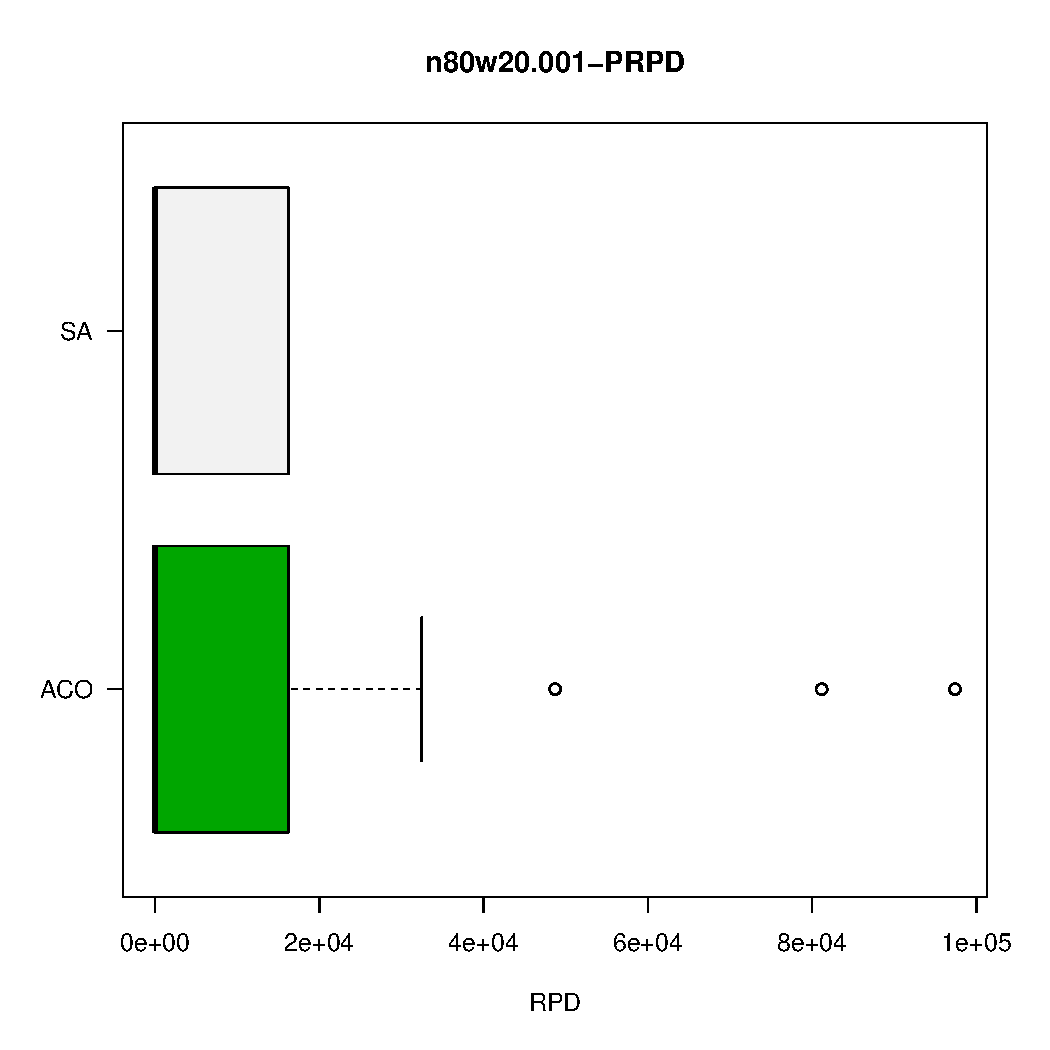
\includegraphics[width=0.6\textwidth,keepaspectratio]{{SLS/n80w20.001/n80w20.001-PRPD}.pdf}
\captionof{figure}{n80w20.001 - Penalised Relative Percentage Deviation box-plot for the implemented SLS algorithms}
\end{center}

\begin{center}
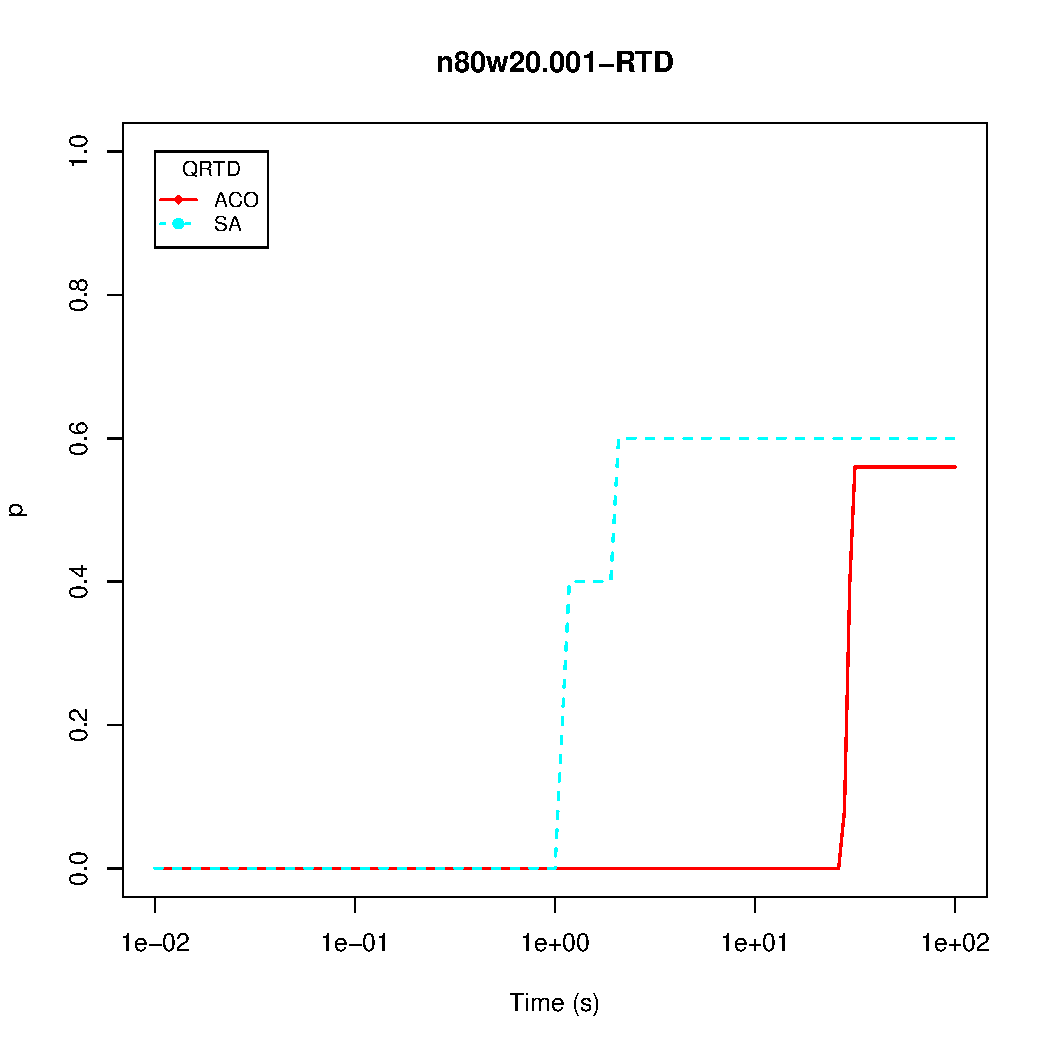
\includegraphics[width=0.6\textwidth,keepaspectratio]{{SLS/n80w20.001/n80w20.001-RTDs}.pdf}
\captionof{figure}{n80w20.001 - Run-time distribution plots of the implemented algorithms for $q* = 0.02$}
\end{center}

\begin{center}
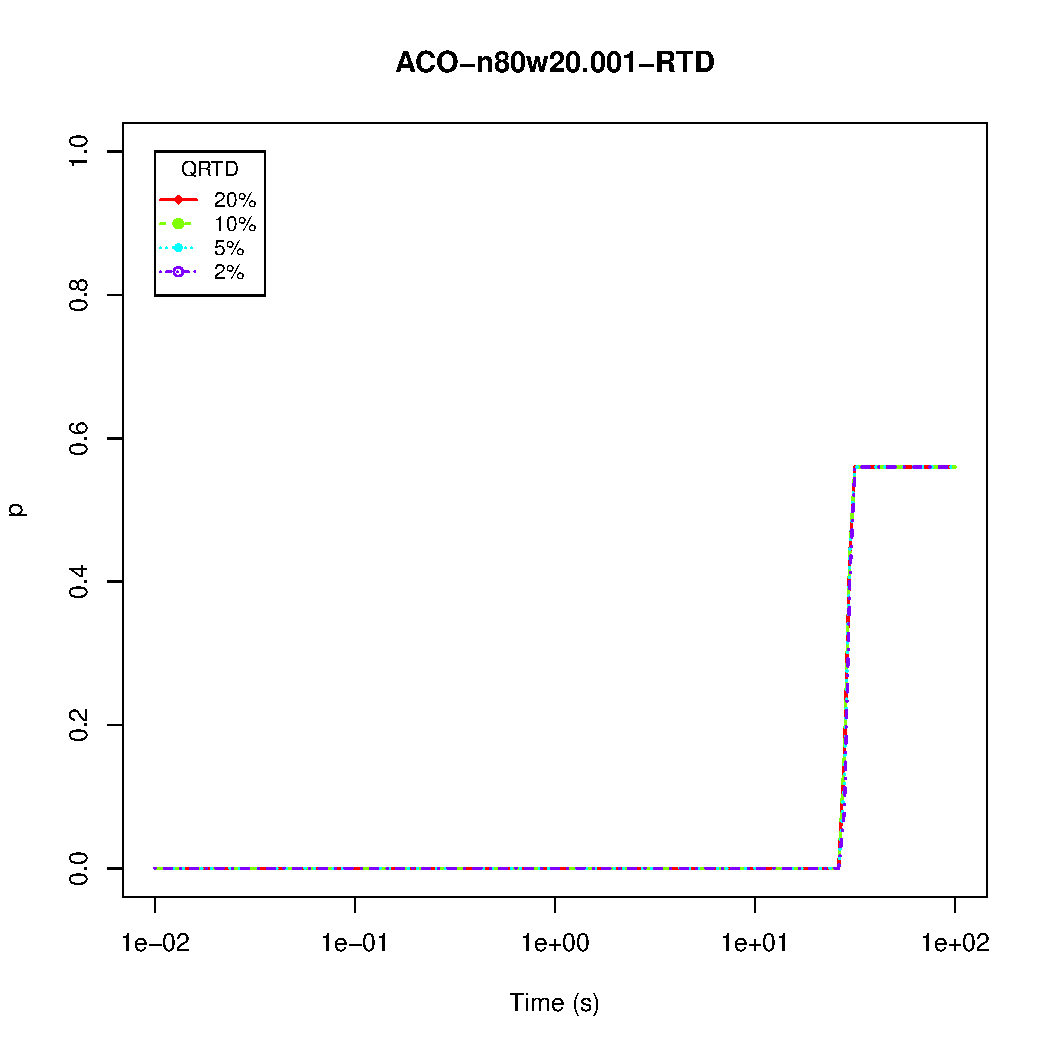
\includegraphics[width=0.6\textwidth,keepaspectratio]{{SLS/n80w20.001/ACO-n80w20.001-RTDs}.pdf}
\captionof{figure}{n80w20.001 - Run-time distribution plots of the ACO algorithm for different values of $q*$}
\end{center}

\begin{center}
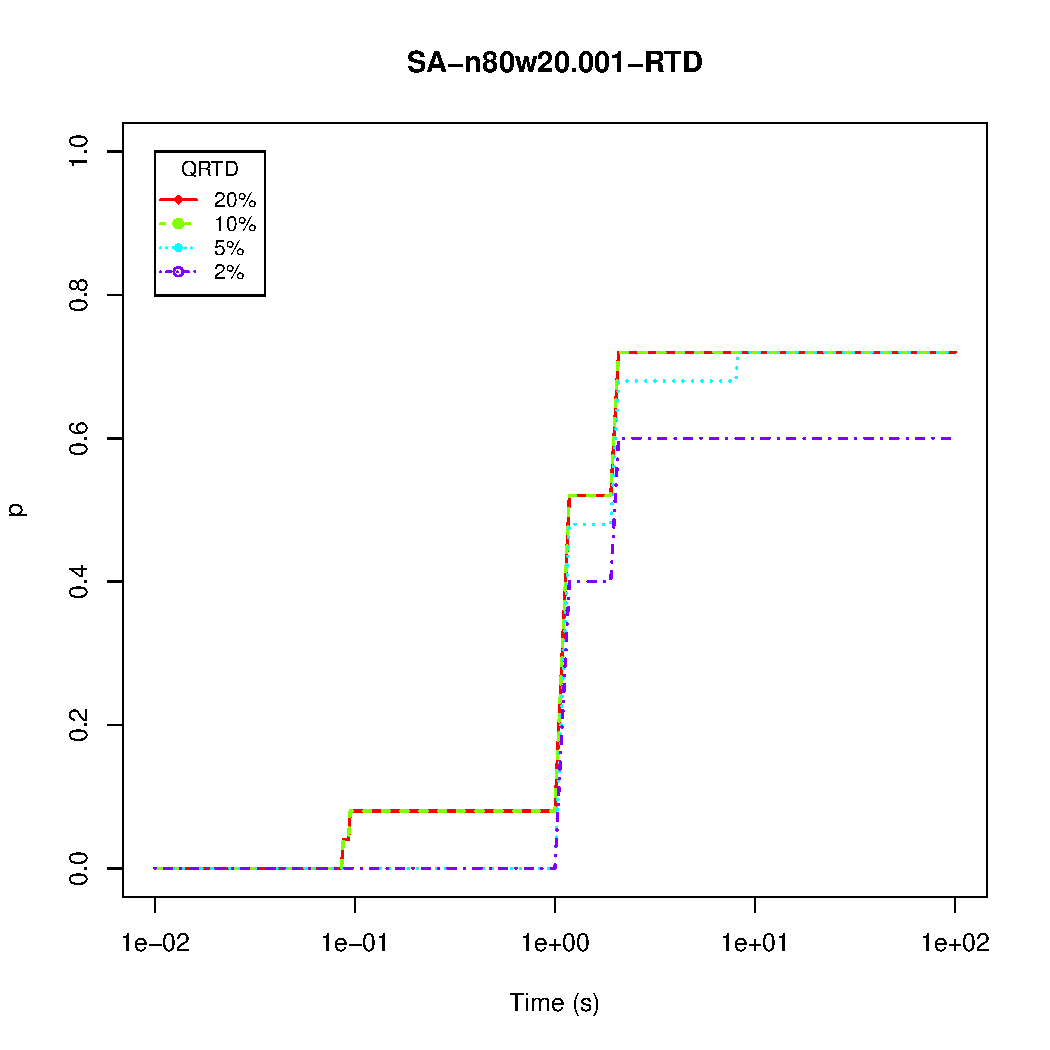
\includegraphics[width=0.6\textwidth,keepaspectratio]{{SLS/n80w20.001/SA-n80w20.001-RTDs}.pdf}
\captionof{figure}{n80w20.001 - Run-time distribution plots of the SA algorithm for different values of $q*$}
\end{center}

\subsubsection{n80w20.002}
\begin{center}
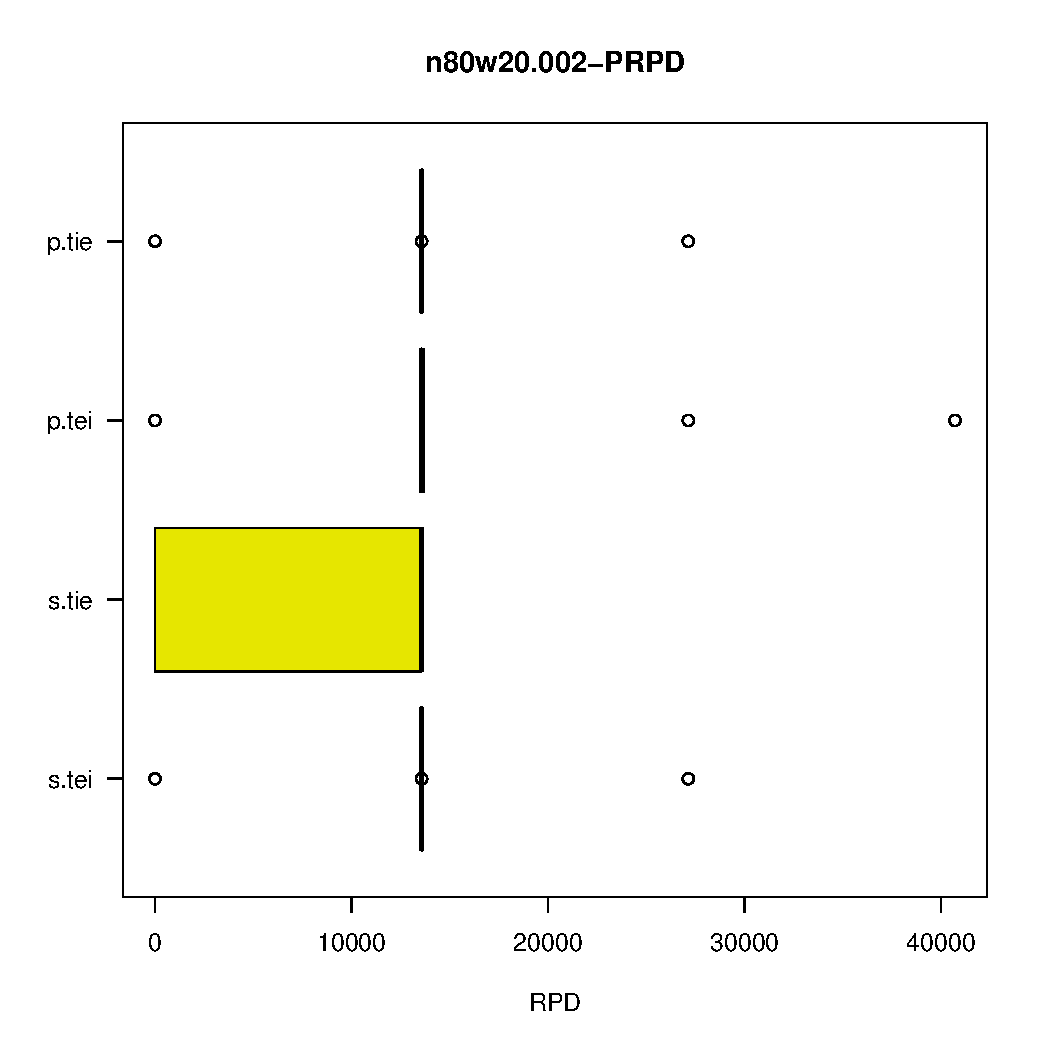
\includegraphics[width=0.6\textwidth,keepaspectratio]{{SLS/n80w20.002/n80w20.002-PRPD}.pdf}
\captionof{figure}{n80w20.002 - Penalised Relative Percentage Deviation box-plot for the implemented SLS algorithms}
\end{center}

\begin{center}
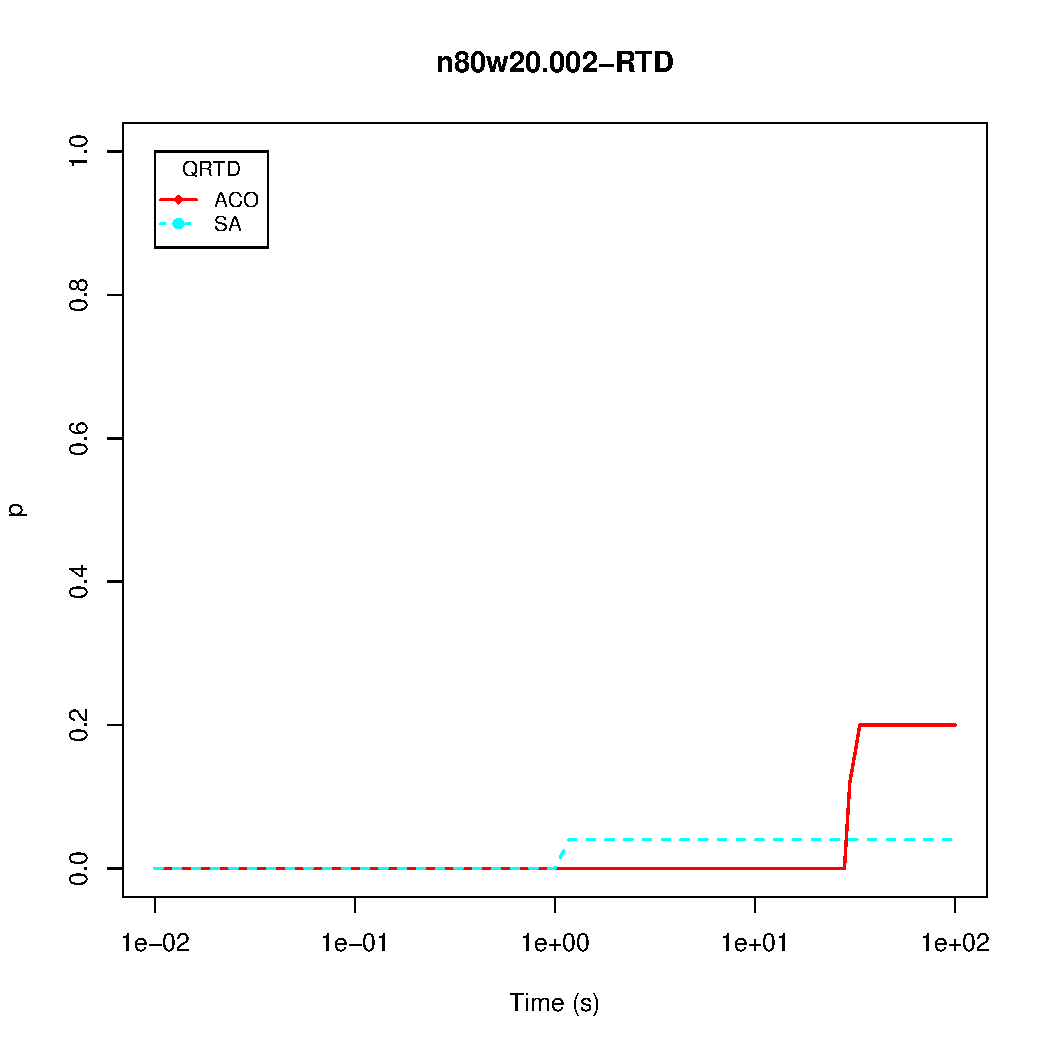
\includegraphics[width=0.6\textwidth,keepaspectratio]{{SLS/n80w20.002/n80w20.002-RTDs}.pdf}
\captionof{figure}{n80w20.002 - Run-time distribution plots of the implemented algorithms for $q* = 0.02$}
\end{center}

\begin{center}
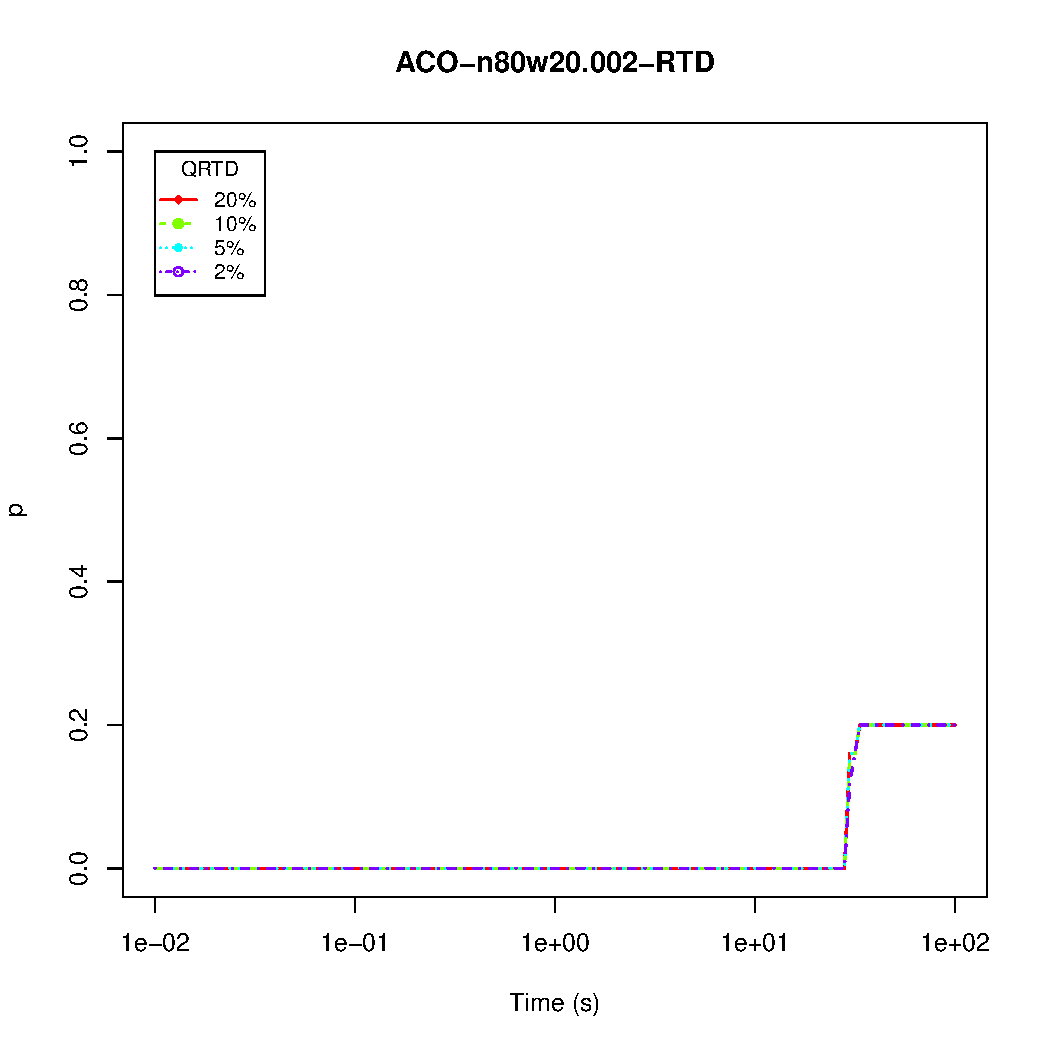
\includegraphics[width=0.6\textwidth,keepaspectratio]{{SLS/n80w20.002/ACO-n80w20.002-RTDs}.pdf}
\captionof{figure}{n80w20.002 - Run-time distribution plots of the ACO algorithm for different values of $q*$}
\end{center}

\begin{center}
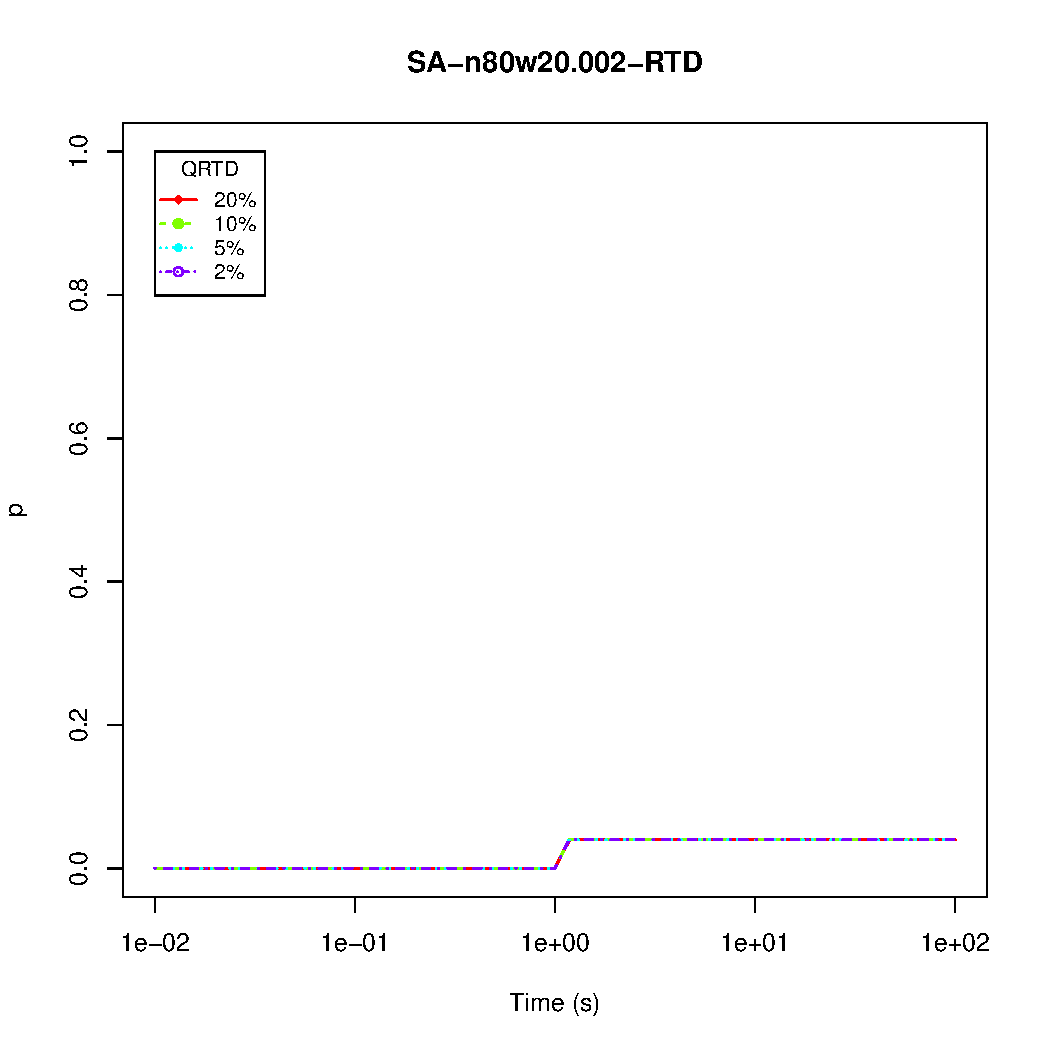
\includegraphics[width=0.6\textwidth,keepaspectratio]{{SLS/n80w20.002/SA-n80w20.002-RTDs}.pdf}
\captionof{figure}{n80w20.002 - Run-time distribution plots of the SA algorithm for different values of $q*$}
\end{center}

\subsubsection{n80w20.003}
\begin{center}
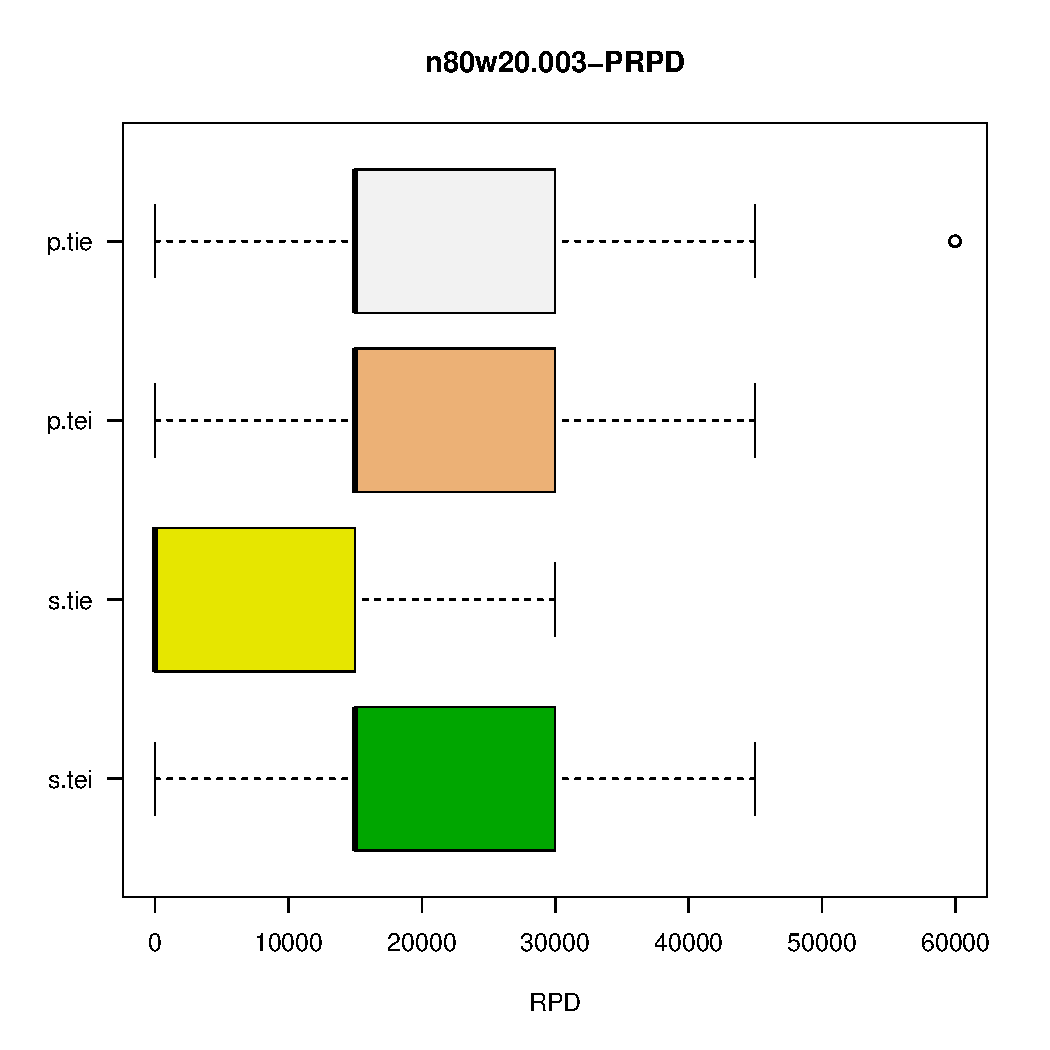
\includegraphics[width=0.6\textwidth,keepaspectratio]{{SLS/n80w20.003/n80w20.003-PRPD}.pdf}
\captionof{figure}{n80w20.003 - Penalised Relative Percentage Deviation box-plot for the implemented SLS algorithms}
\end{center}

\begin{center}
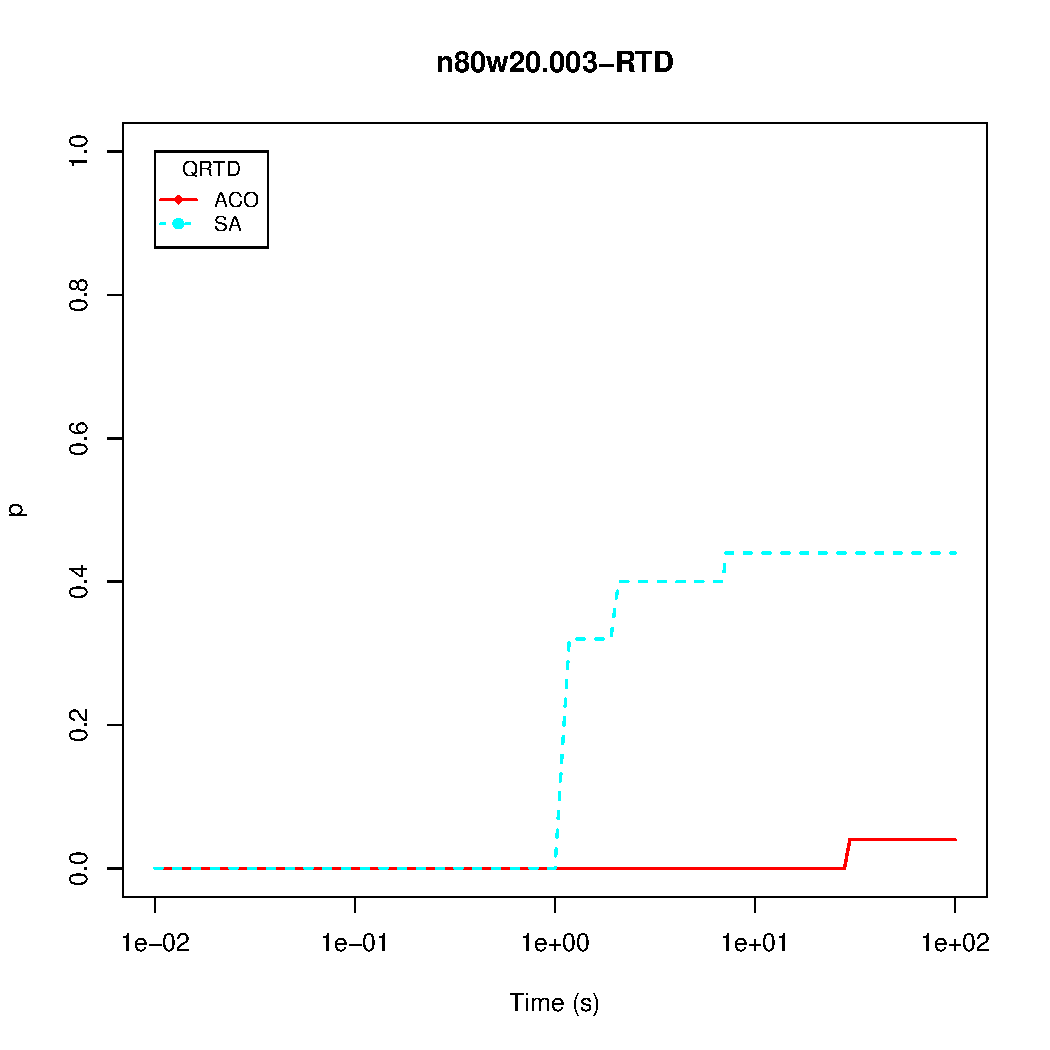
\includegraphics[width=0.6\textwidth,keepaspectratio]{{SLS/n80w20.003/n80w20.003-RTDs}.pdf}
\captionof{figure}{n80w20.003 - Run-time distribution plots of the implemented algorithms for $q* = 0.02$}
\end{center}

\begin{center}
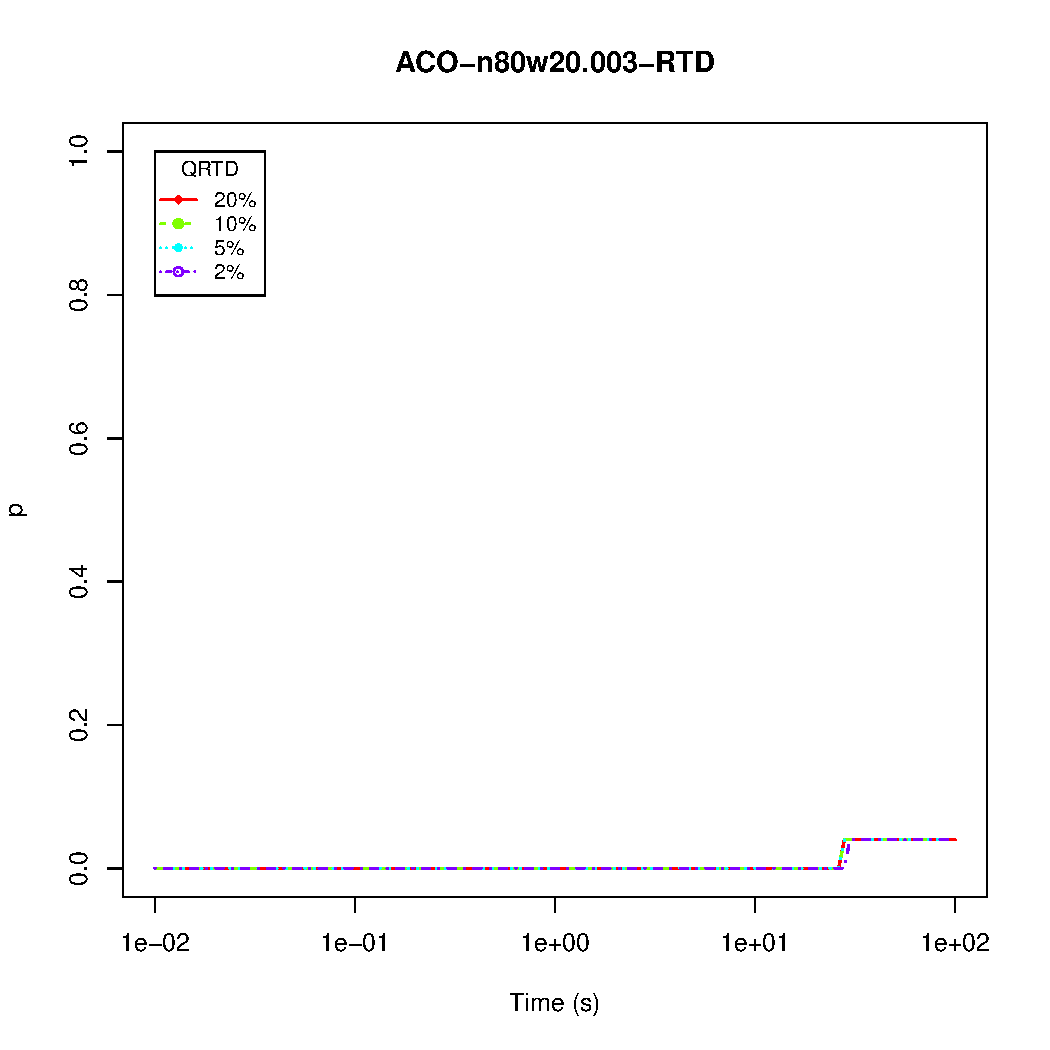
\includegraphics[width=0.6\textwidth,keepaspectratio]{{SLS/n80w20.003/ACO-n80w20.003-RTDs}.pdf}
\captionof{figure}{n80w20.003 - Run-time distribution plots of the ACO algorithm for different values of $q*$}
\end{center}

\begin{center}
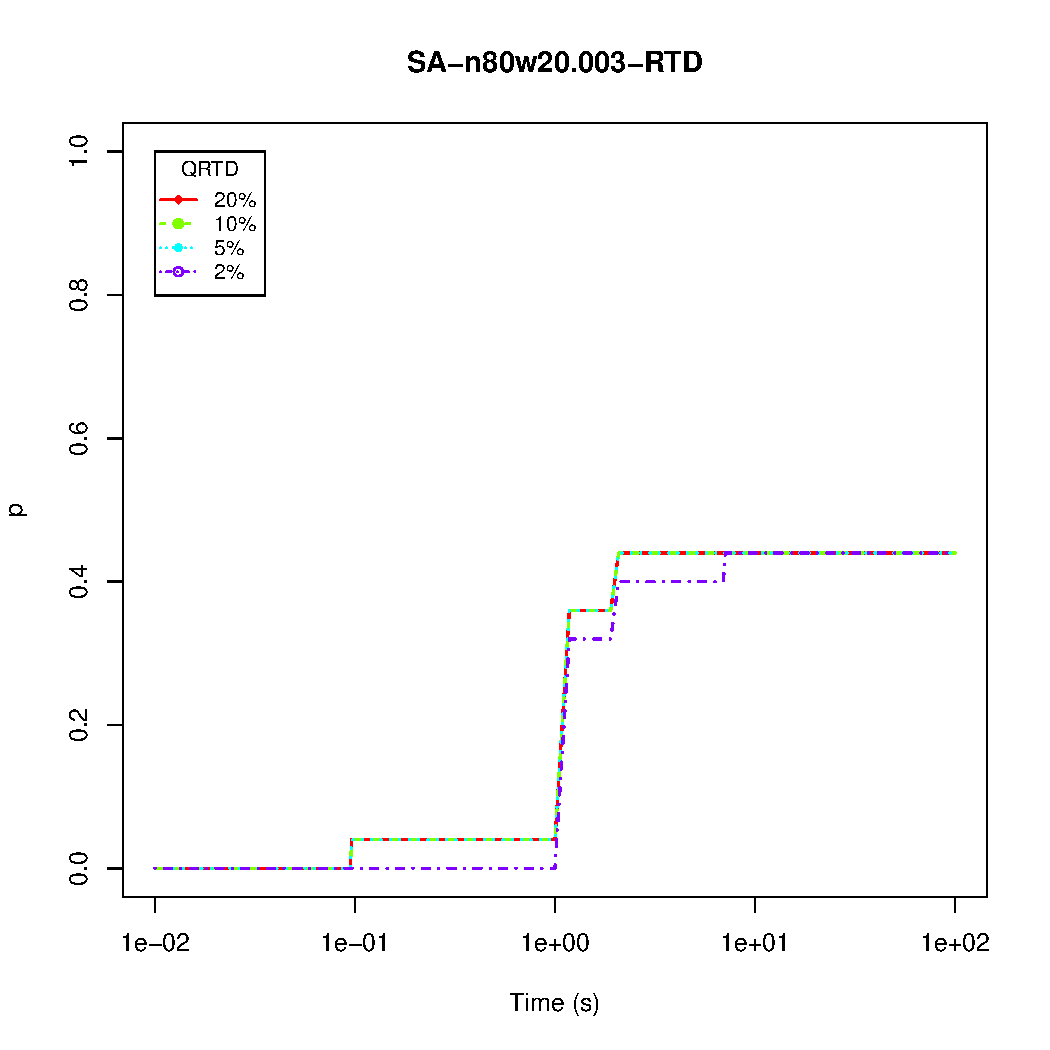
\includegraphics[width=0.6\textwidth,keepaspectratio]{{SLS/n80w20.003/SA-n80w20.003-RTDs}.pdf}
\captionof{figure}{n80w20.003 - Run-time distribution plots of the SA algorithm for different values of $q*$}
\end{center}

\subsubsection{n80w20.004}
\begin{center}
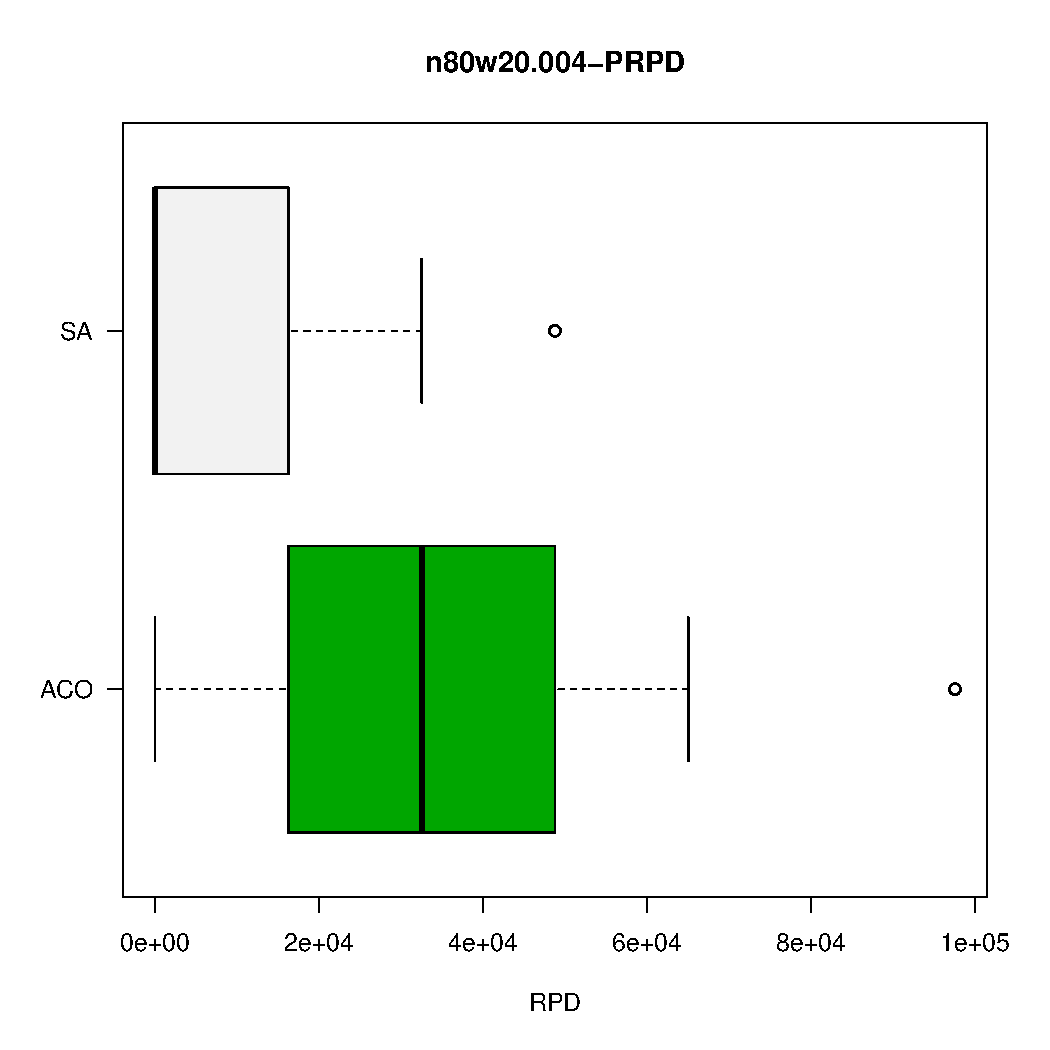
\includegraphics[width=0.6\textwidth,keepaspectratio]{{SLS/n80w20.004/n80w20.004-PRPD}.pdf}
\captionof{figure}{n80w20.004 - Penalised Relative Percentage Deviation box-plot for the implemented SLS algorithms}
\end{center}

\begin{center}
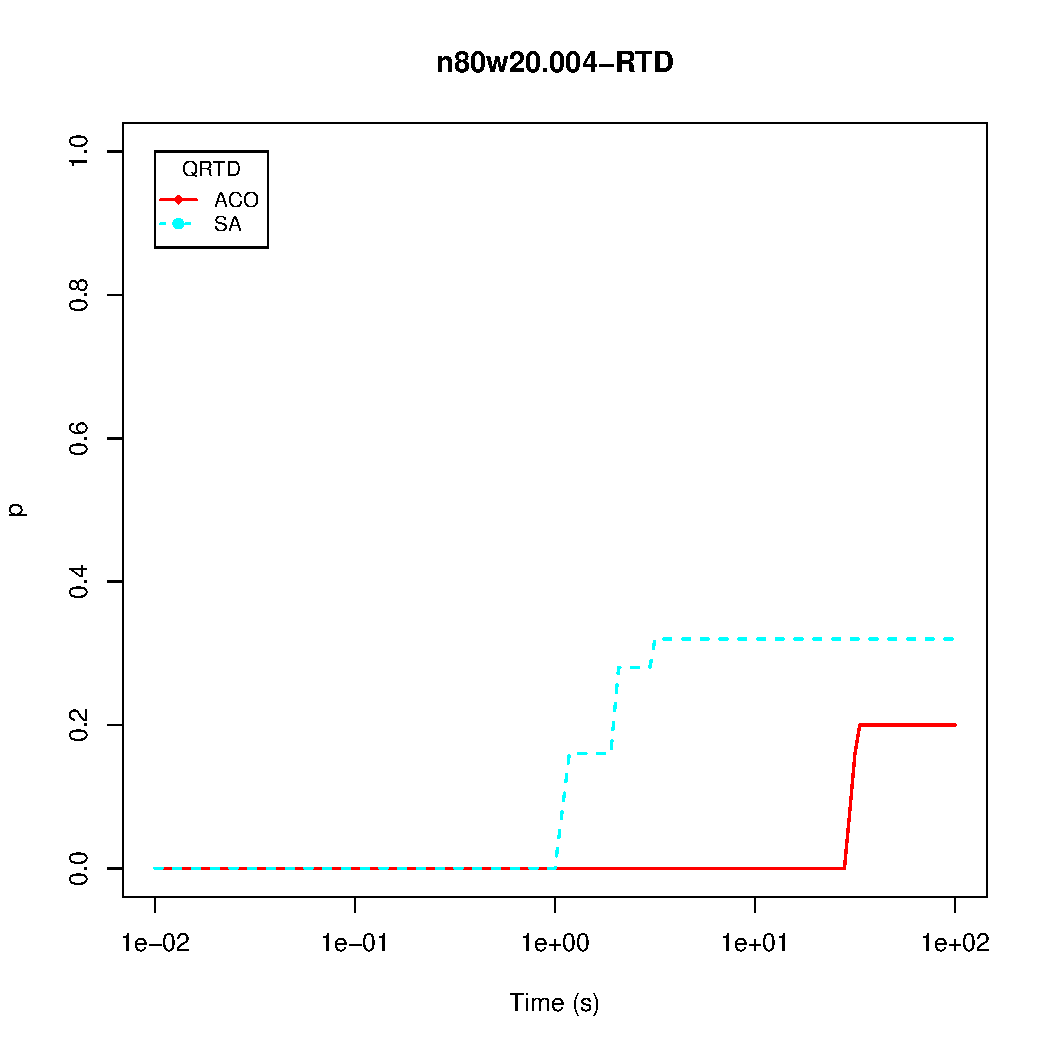
\includegraphics[width=0.6\textwidth,keepaspectratio]{{SLS/n80w20.004/n80w20.004-RTDs}.pdf}
\captionof{figure}{n80w20.004 - Run-time distribution plots of the implemented algorithms for $q* = 0.02$}
\end{center}

\begin{center}
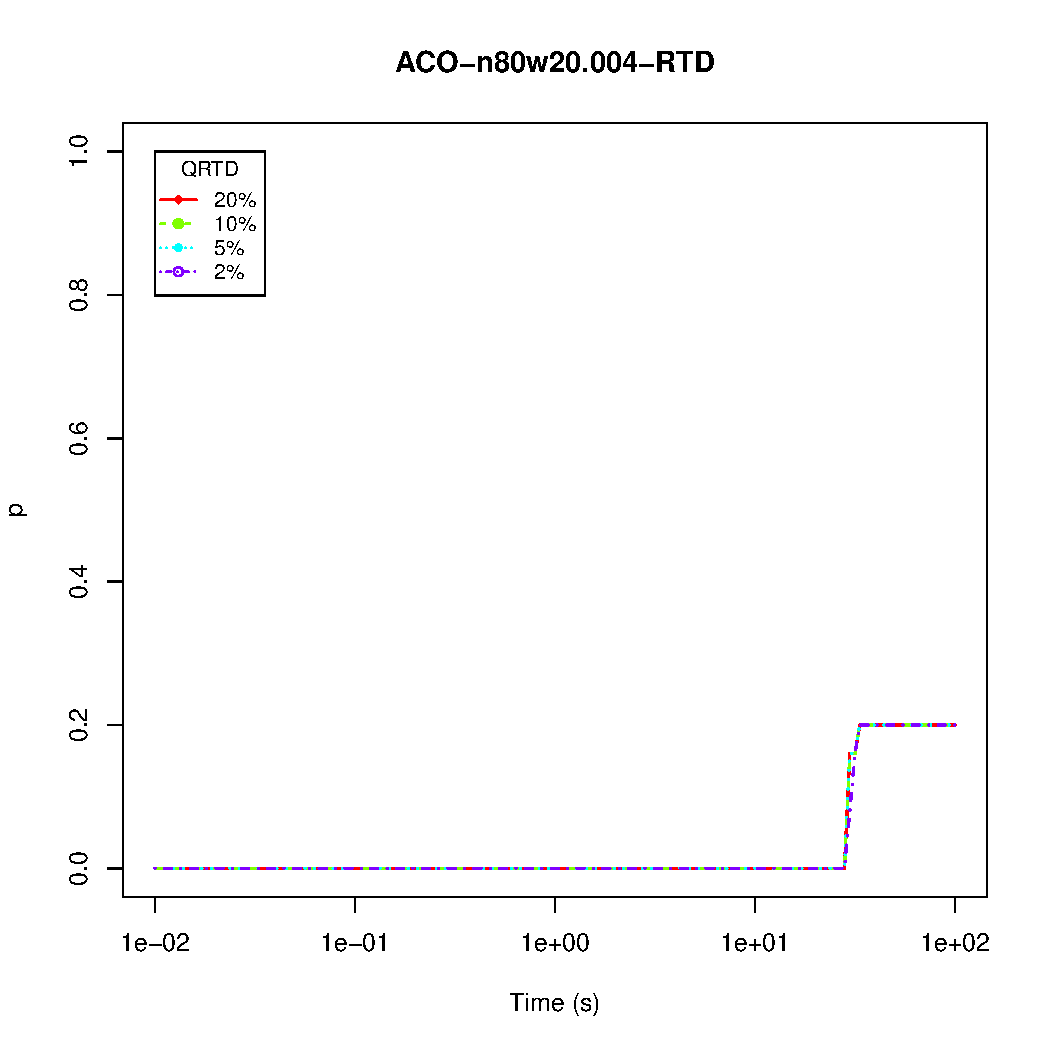
\includegraphics[width=0.6\textwidth,keepaspectratio]{{SLS/n80w20.004/ACO-n80w20.004-RTDs}.pdf}
\captionof{figure}{n80w20.004 - Run-time distribution plots of the ACO algorithm for different values of $q*$}
\end{center}

\begin{center}
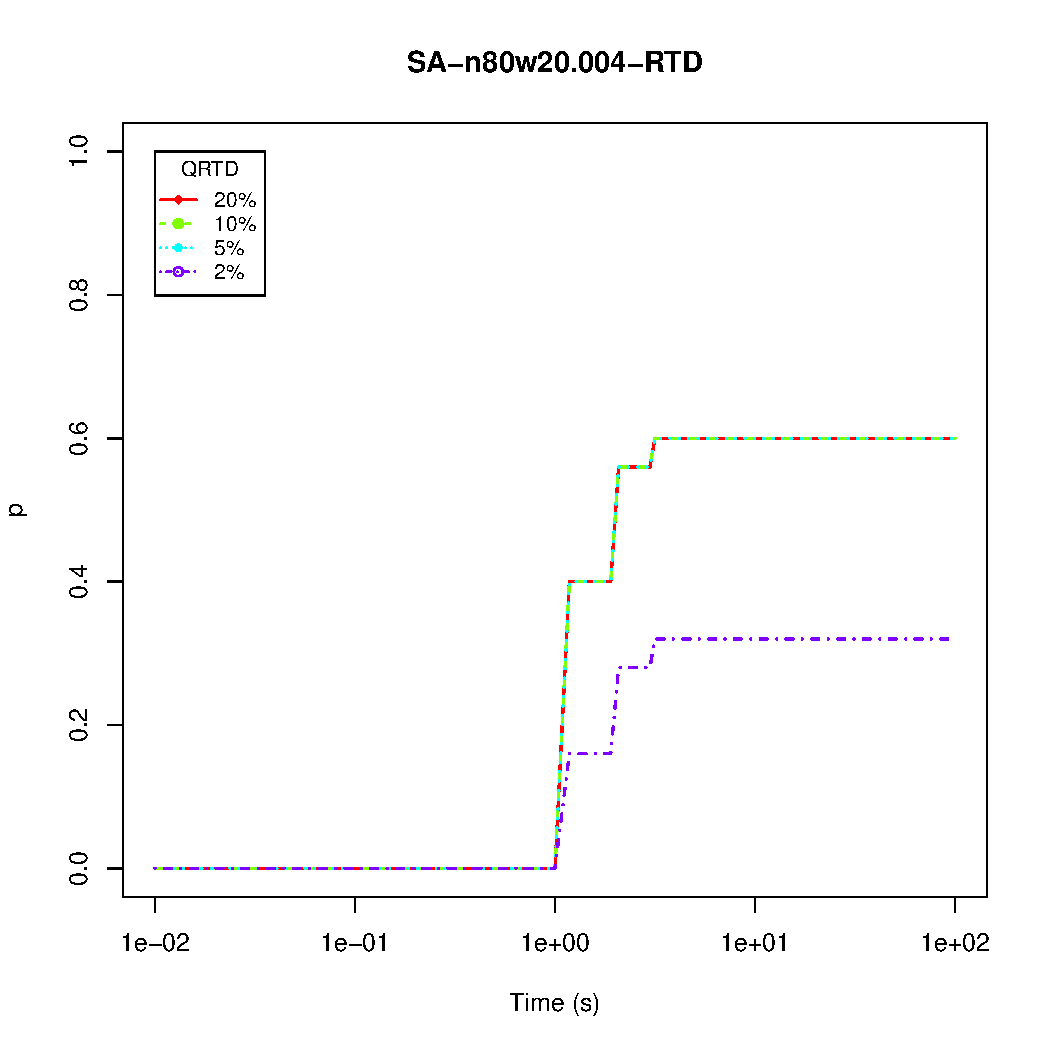
\includegraphics[width=0.6\textwidth,keepaspectratio]{{SLS/n80w20.004/SA-n80w20.004-RTDs}.pdf}
\captionof{figure}{n80w20.004 - Run-time distribution plots of the SA algorithm for different values of $q*$}
\end{center}

\subsubsection{n80w20.005}
\begin{center}
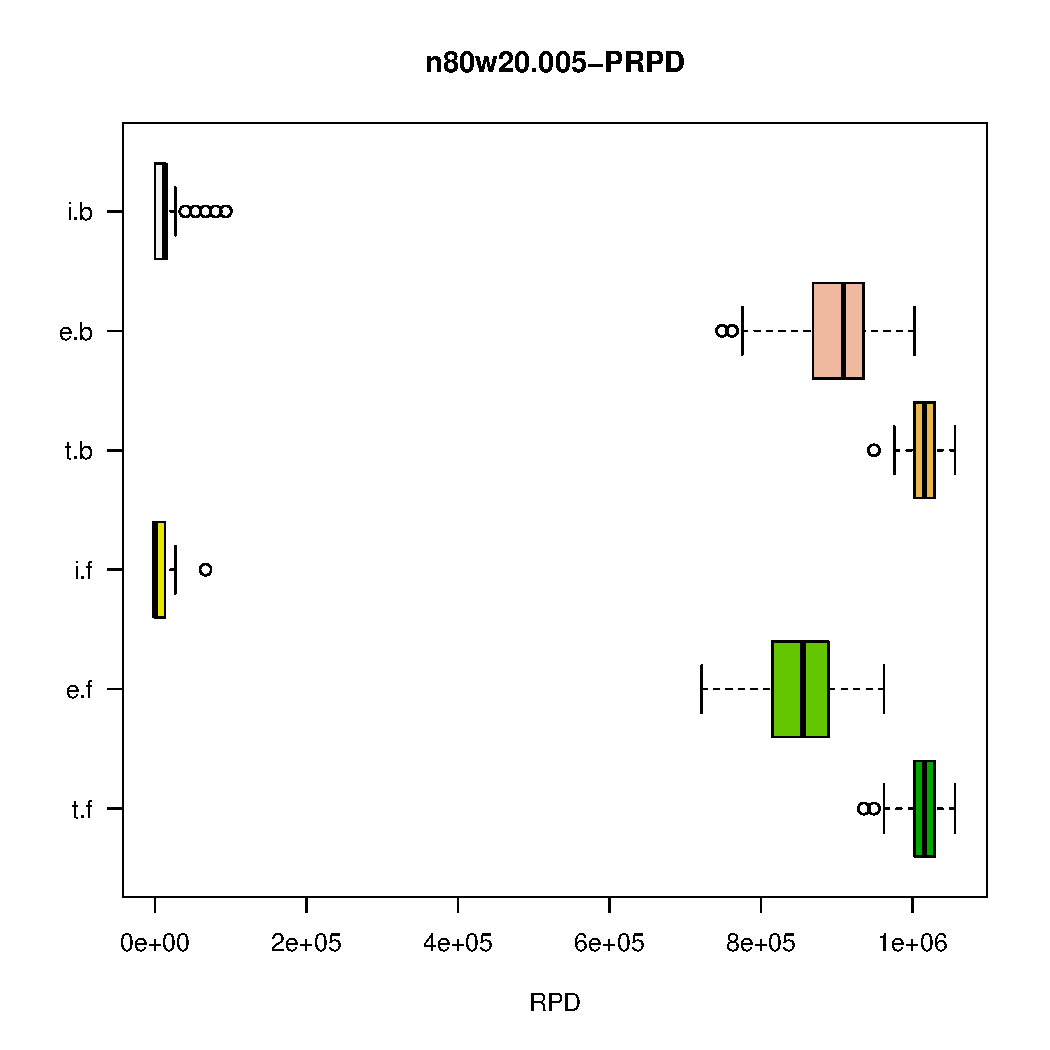
\includegraphics[width=0.6\textwidth,keepaspectratio]{{SLS/n80w20.005/n80w20.005-PRPD}.pdf}
\captionof{figure}{n80w20.005 - Penalised Relative Percentage Deviation box-plot for the implemented SLS algorithms}
\end{center}

\begin{center}
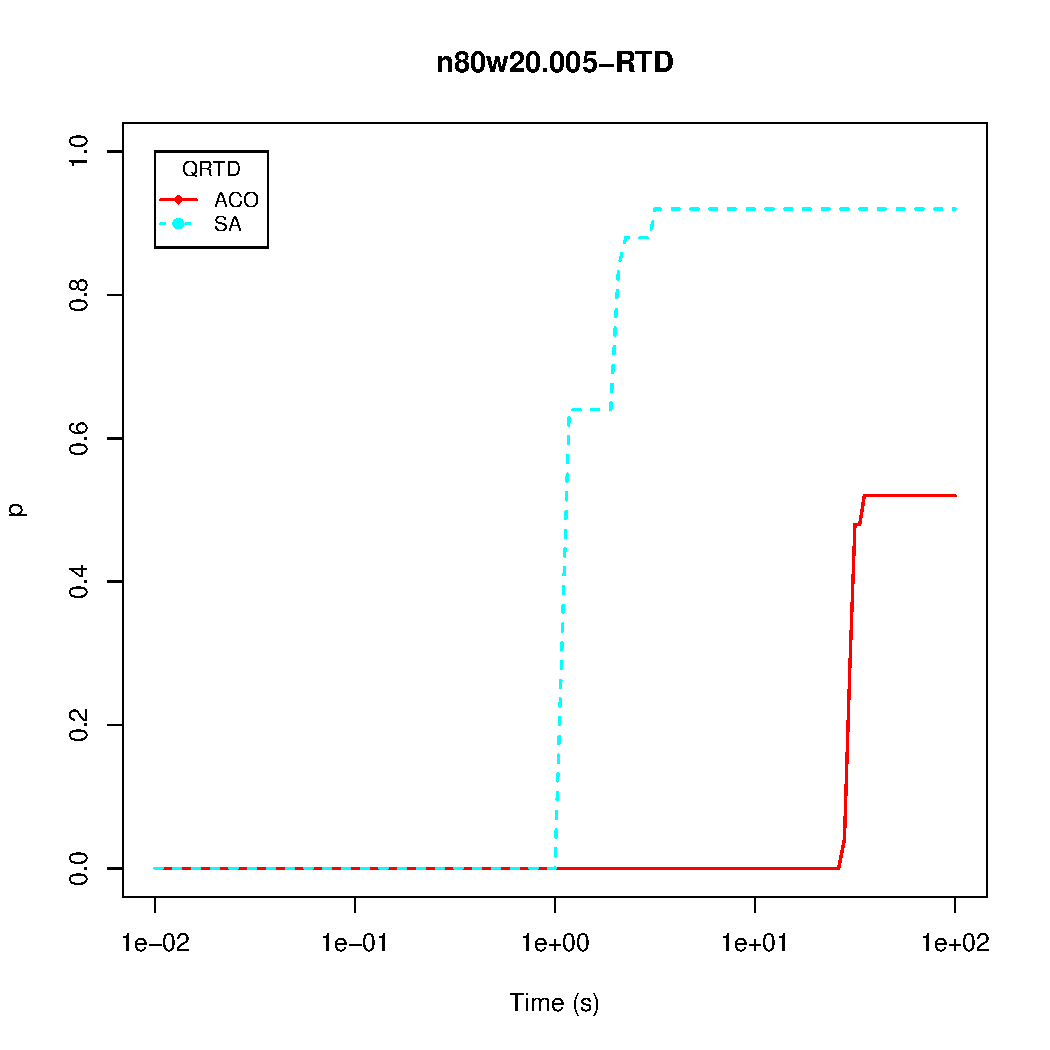
\includegraphics[width=0.6\textwidth,keepaspectratio]{{SLS/n80w20.005/n80w20.005-RTDs}.pdf}
\captionof{figure}{n80w20.005 - Run-time distribution plots of the implemented algorithms for $q* = 0.02$}
\end{center}

\begin{center}
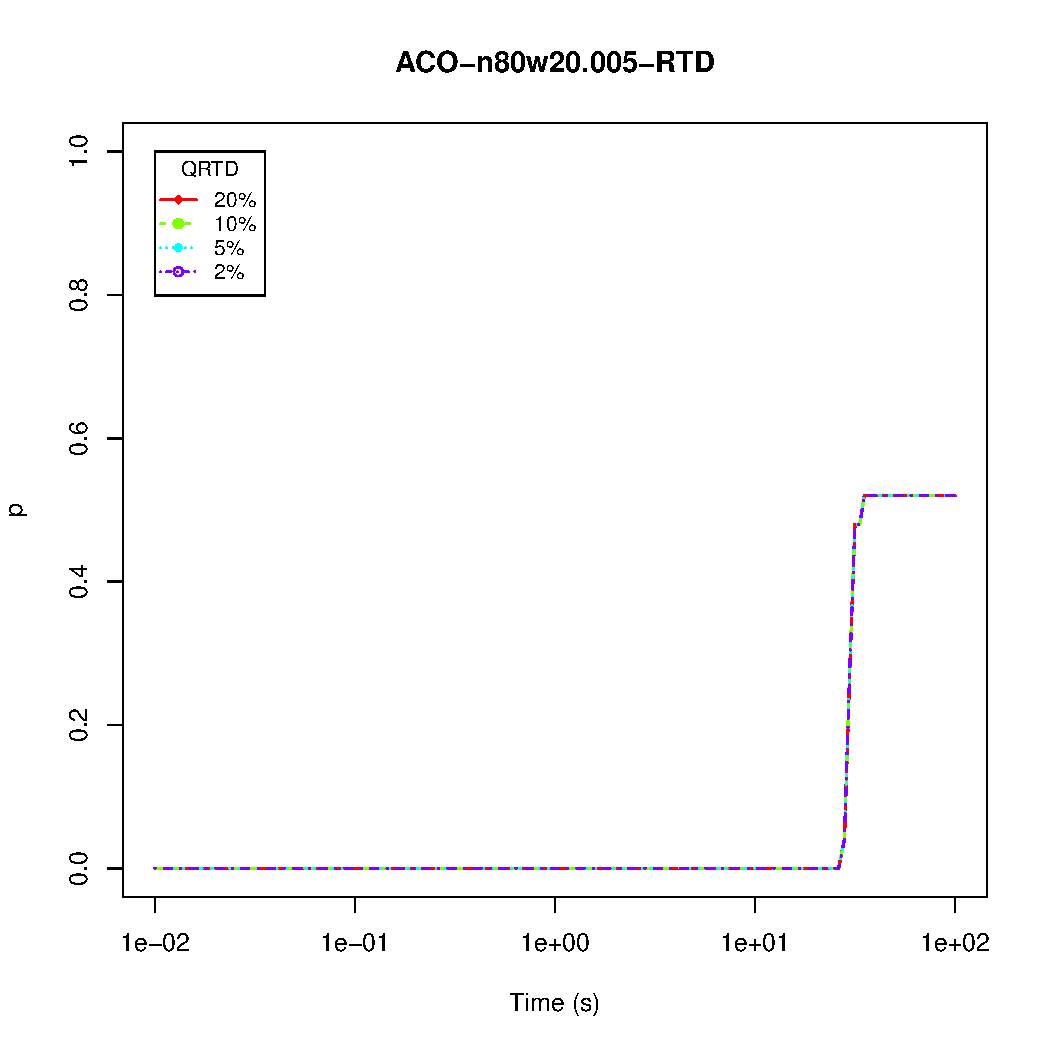
\includegraphics[width=0.6\textwidth,keepaspectratio]{{SLS/n80w20.005/ACO-n80w20.005-RTDs}.pdf}
\captionof{figure}{n80w20.005 - Run-time distribution plots of the ACO algorithm for different values of $q*$}
\end{center}

\begin{center}
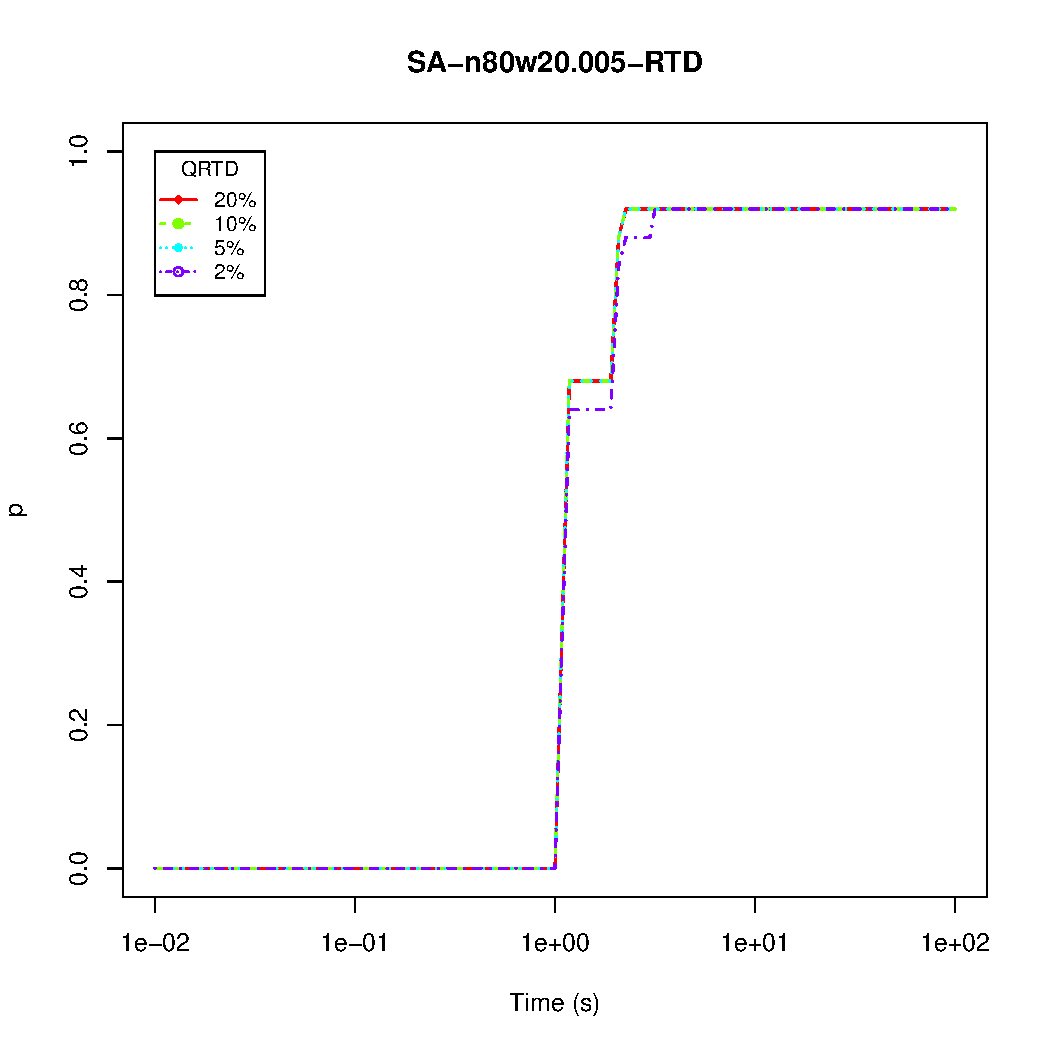
\includegraphics[width=0.6\textwidth,keepaspectratio]{{SLS/n80w20.005/SA-n80w20.005-RTDs}.pdf}
\captionof{figure}{n80w20.005 - Run-time distribution plots of the SA algorithm for different values of $q*$}
\end{center}

\subsubsection{n80w200.001}
\begin{center}
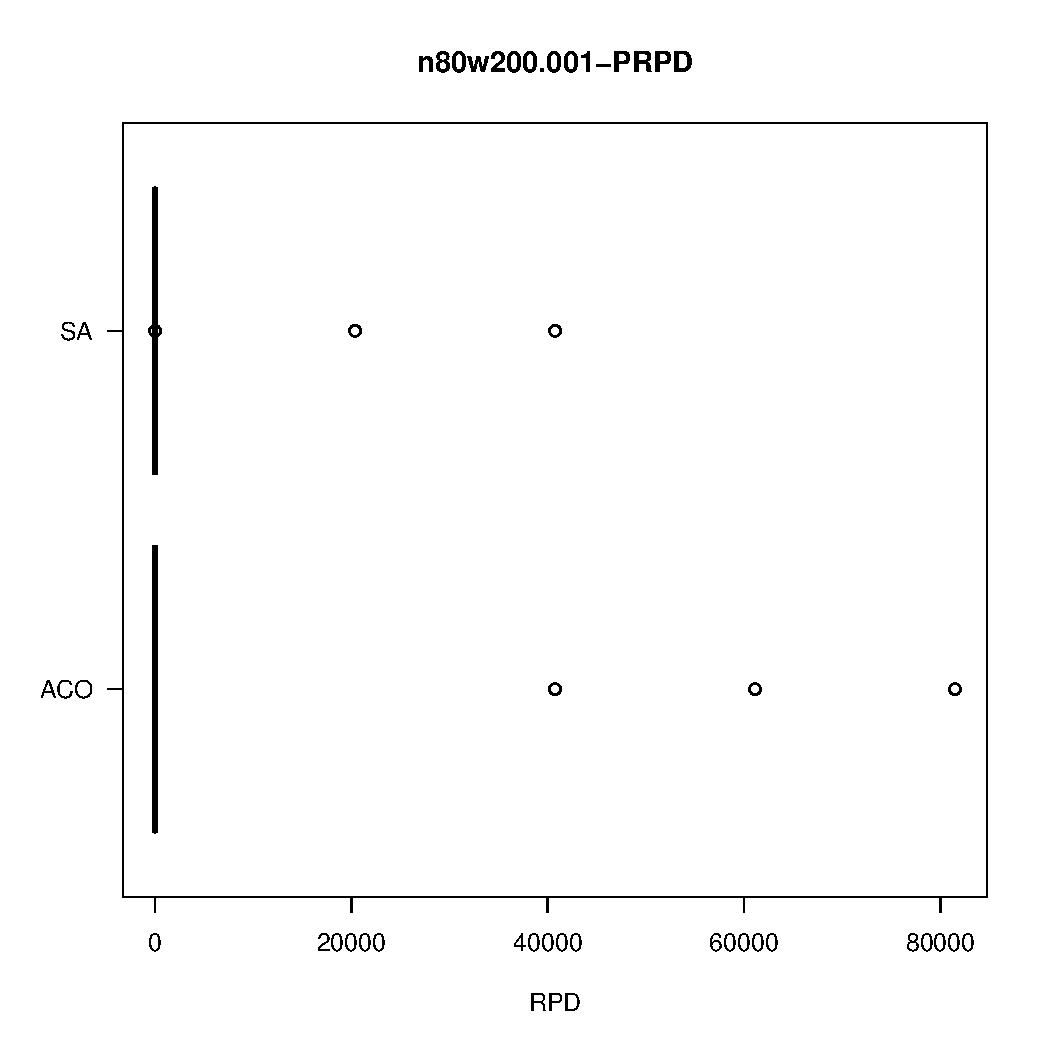
\includegraphics[width=0.6\textwidth,keepaspectratio]{{SLS/n80w200.001/n80w200.001-PRPD}.pdf}
\captionof{figure}{n80w200.001 - Penalised Relative Percentage Deviation box-plot for the implemented SLS algorithms}
\end{center}

\begin{center}
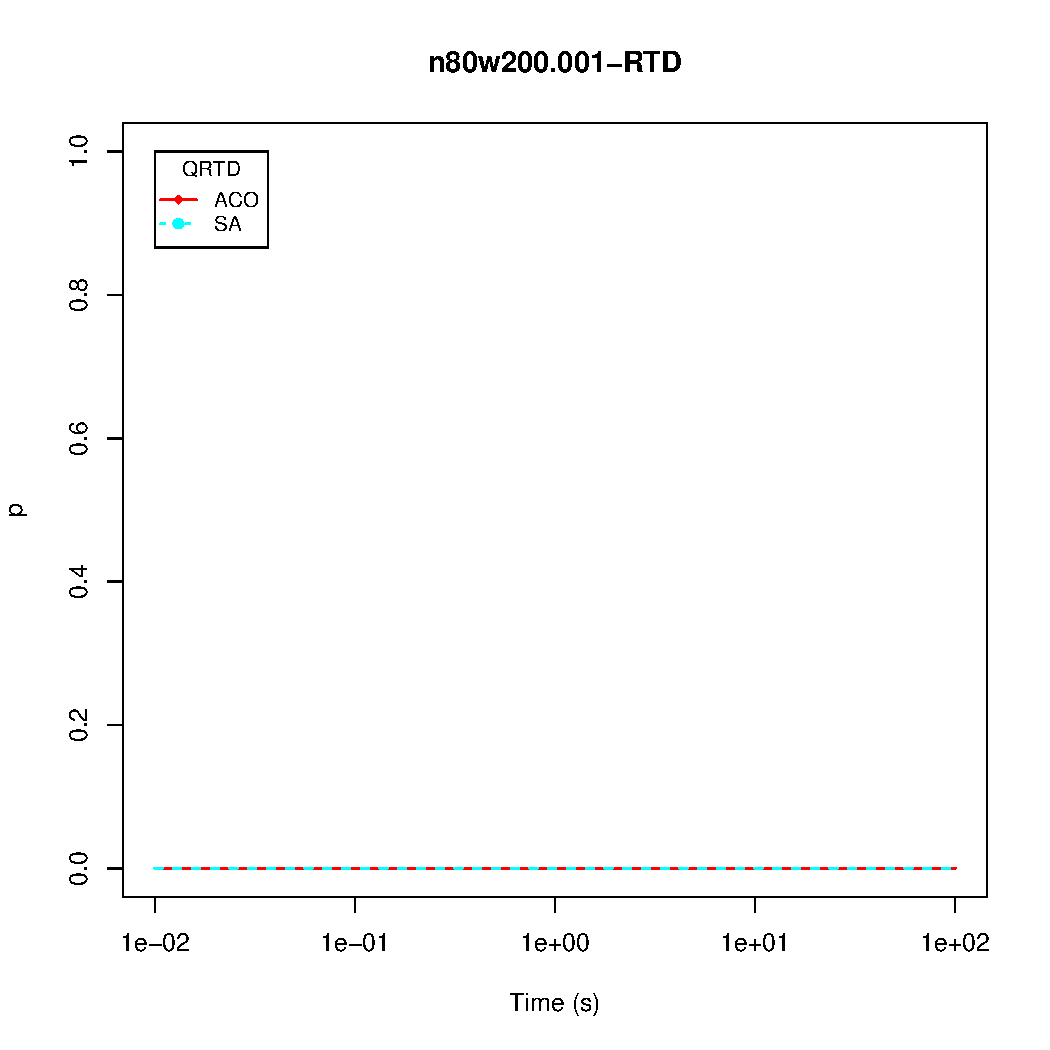
\includegraphics[width=0.6\textwidth,keepaspectratio]{{SLS/n80w200.001/n80w200.001-RTDs}.pdf}
\captionof{figure}{n80w200.001 - Run-time distribution plots of the implemented algorithms for $q* = 0.02$}
\end{center}

\begin{center}
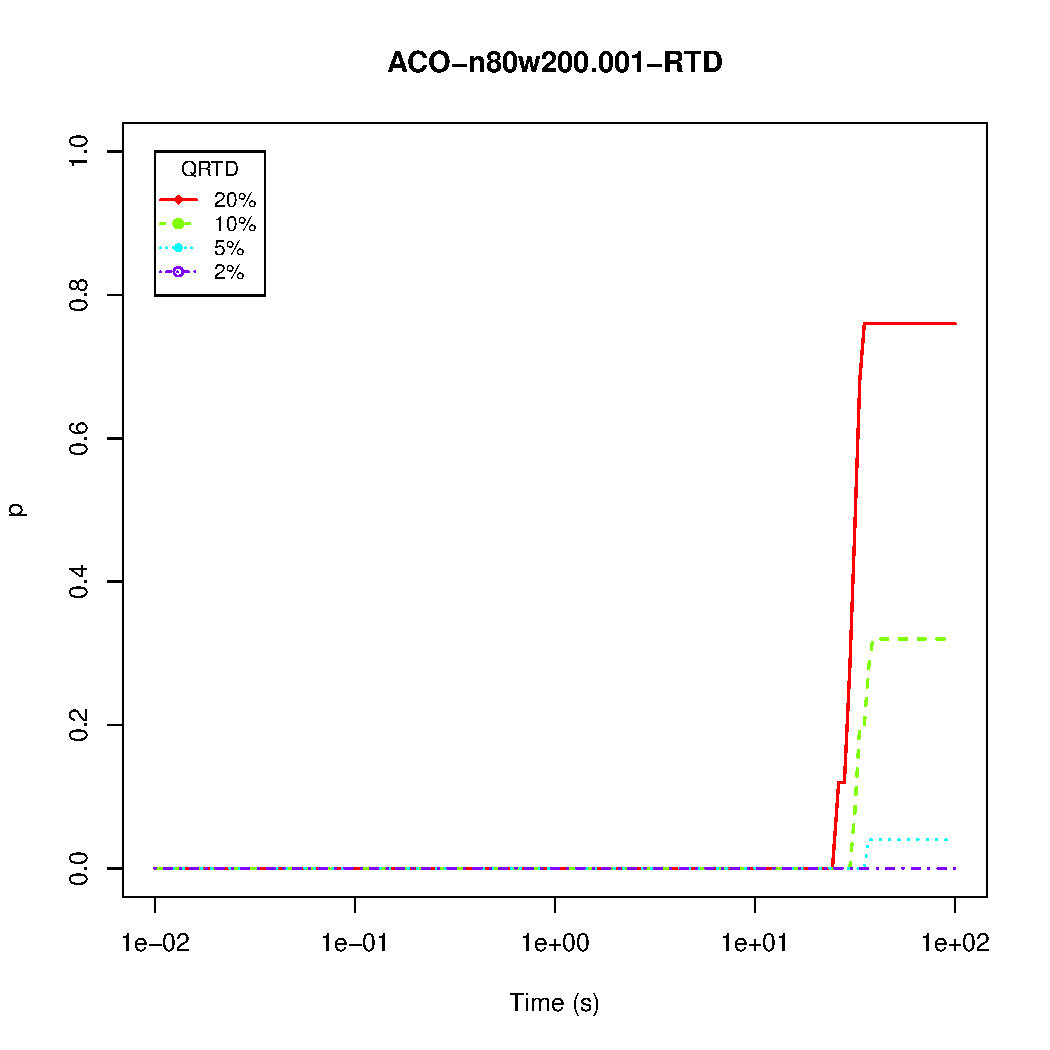
\includegraphics[width=0.6\textwidth,keepaspectratio]{{SLS/n80w200.001/ACO-n80w200.001-RTDs}.pdf}
\captionof{figure}{n80w200.001 - Run-time distribution plots of the ACO algorithm for different values of $q*$}
\end{center}

\begin{center}
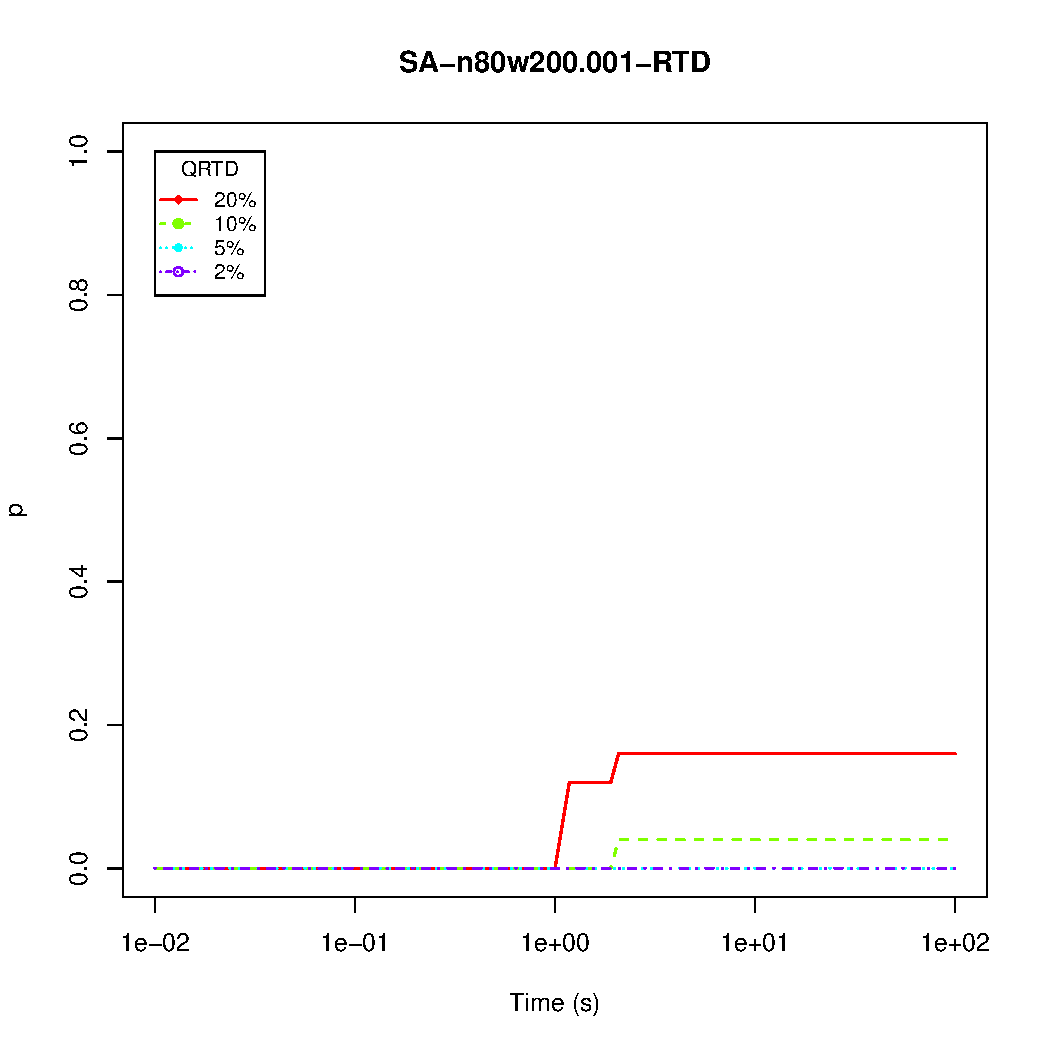
\includegraphics[width=0.6\textwidth,keepaspectratio]{{SLS/n80w200.001/SA-n80w200.001-RTDs}.pdf}
\captionof{figure}{n80w200.001 - Run-time distribution plots of the SA algorithm for different values of $q*$}
\end{center}

\subsubsection{n80w200.002}
\begin{center}
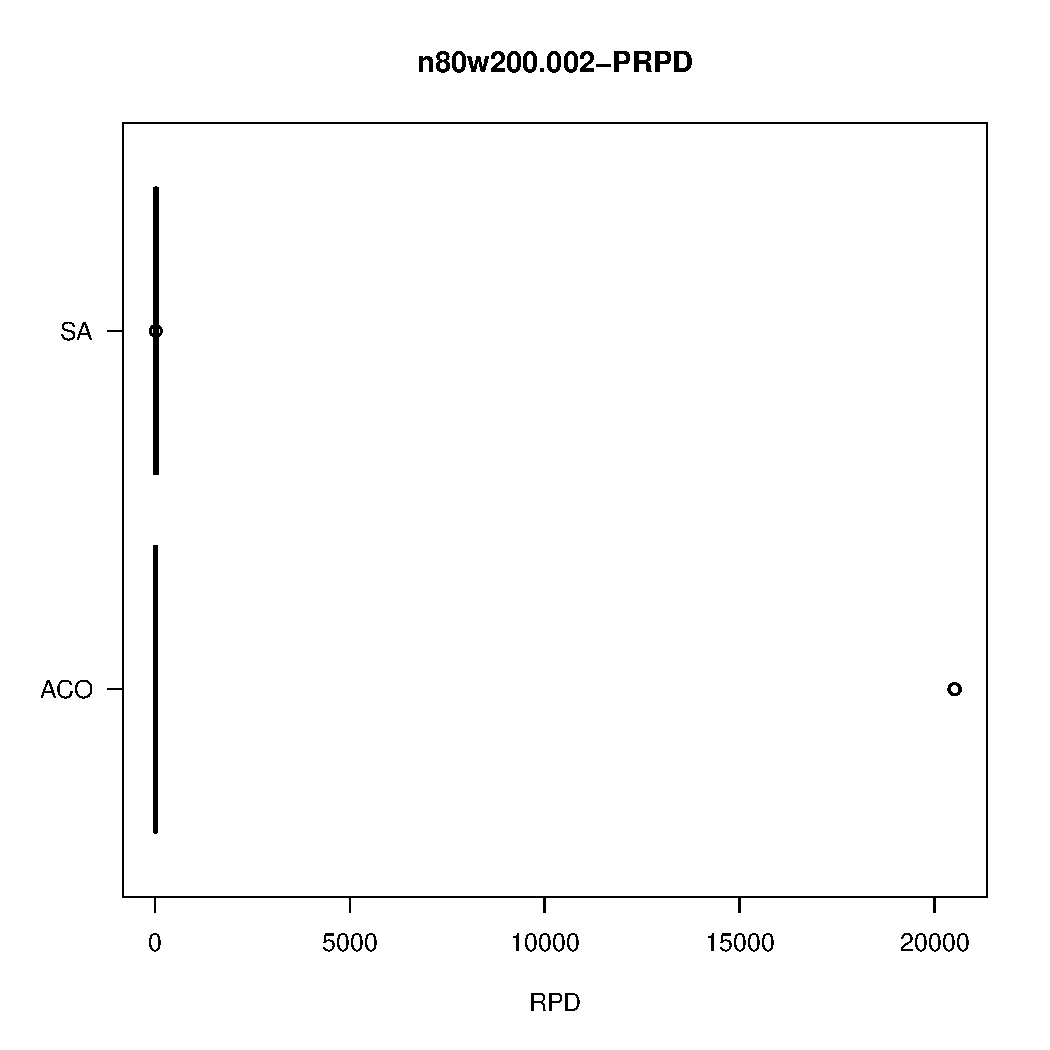
\includegraphics[width=0.6\textwidth,keepaspectratio]{{SLS/n80w200.002/n80w200.002-PRPD}.pdf}
\captionof{figure}{n80w200.002 - Penalised Relative Percentage Deviation box-plot for the implemented SLS algorithms}
\end{center}

\begin{center}
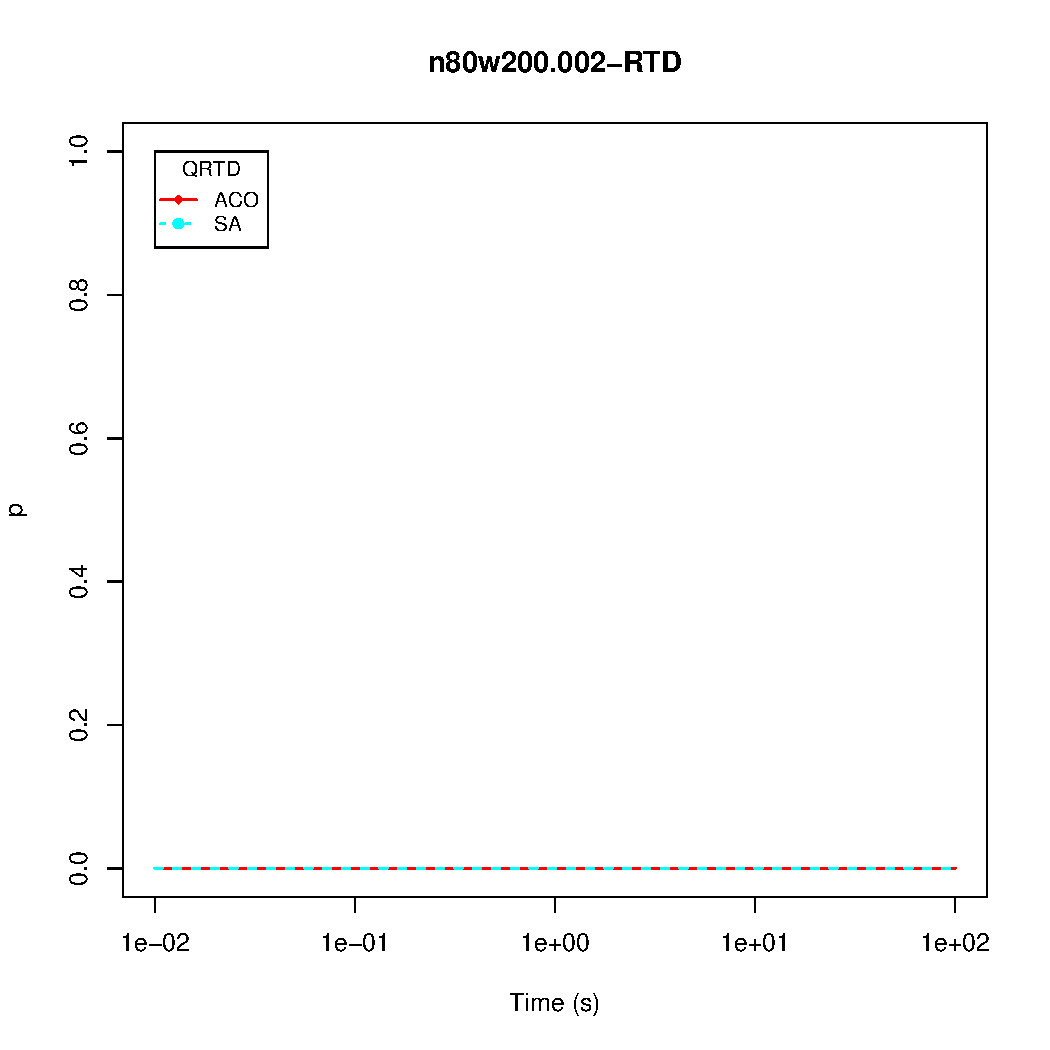
\includegraphics[width=0.6\textwidth,keepaspectratio]{{SLS/n80w200.002/n80w200.002-RTDs}.pdf}
\captionof{figure}{n80w200.002 - Run-time distribution plots of the implemented algorithms for $q* = 0.02$}
\end{center}

\begin{center}
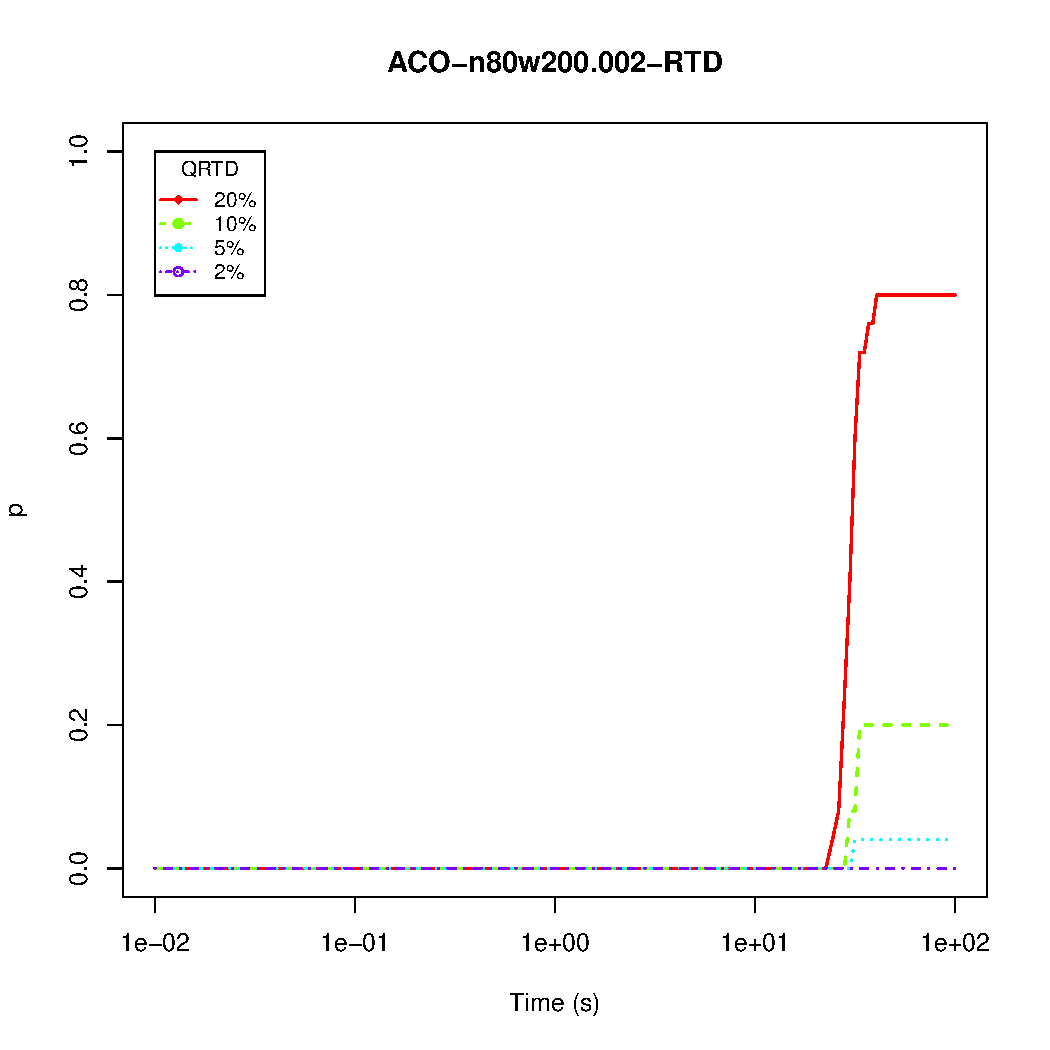
\includegraphics[width=0.6\textwidth,keepaspectratio]{{SLS/n80w200.002/ACO-n80w200.002-RTDs}.pdf}
\captionof{figure}{n80w200.002 - Run-time distribution plots of the ACO algorithm for different values of $q*$}
\end{center}

\begin{center}
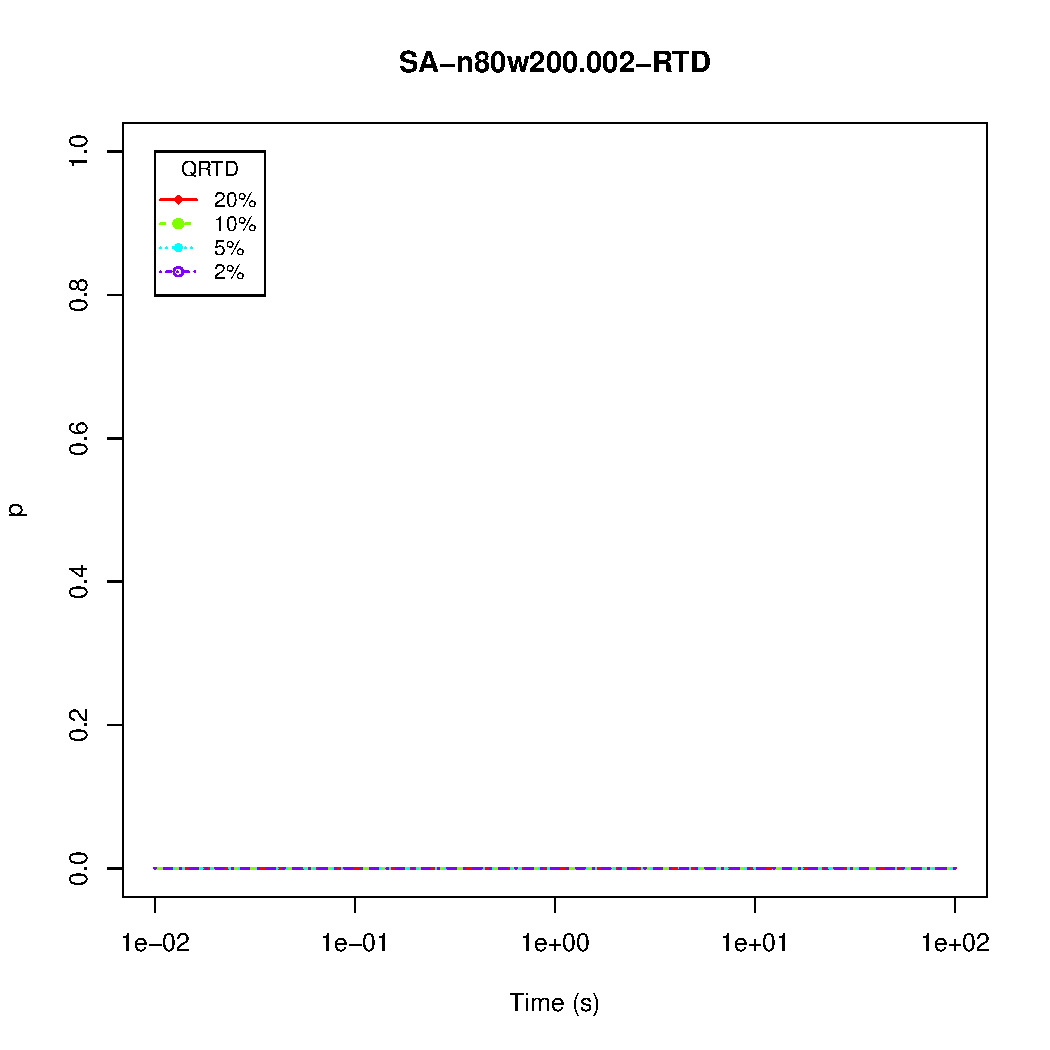
\includegraphics[width=0.6\textwidth,keepaspectratio]{{SLS/n80w200.002/SA-n80w200.002-RTDs}.pdf}
\captionof{figure}{n80w200.002 - Run-time distribution plots of the SA algorithm for different values of $q*$}
\end{center}

\subsubsection{n80w200.003}
\begin{center}
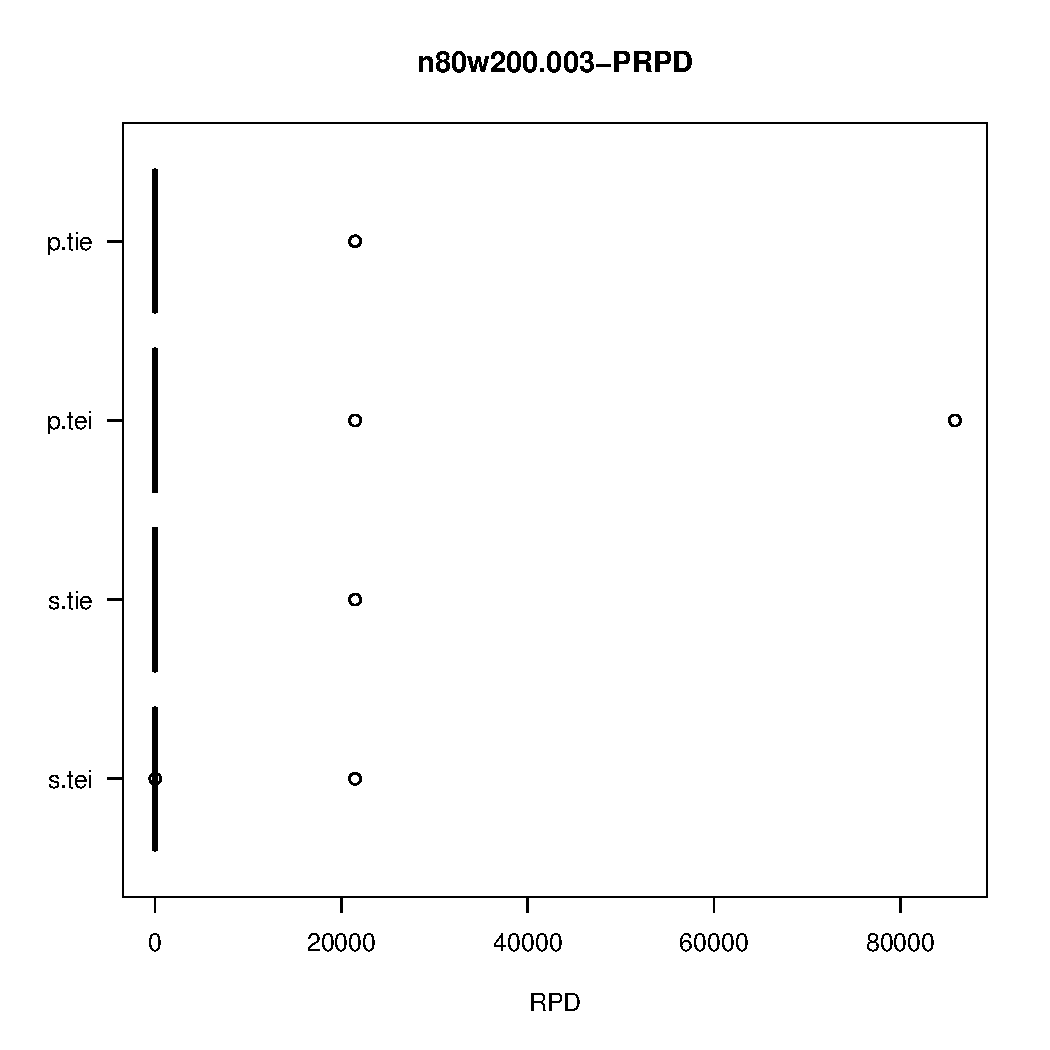
\includegraphics[width=0.6\textwidth,keepaspectratio]{{SLS/n80w200.003/n80w200.003-PRPD}.pdf}
\captionof{figure}{n80w200.003 - Penalised Relative Percentage Deviation box-plot for the implemented SLS algorithms}
\end{center}

\begin{center}
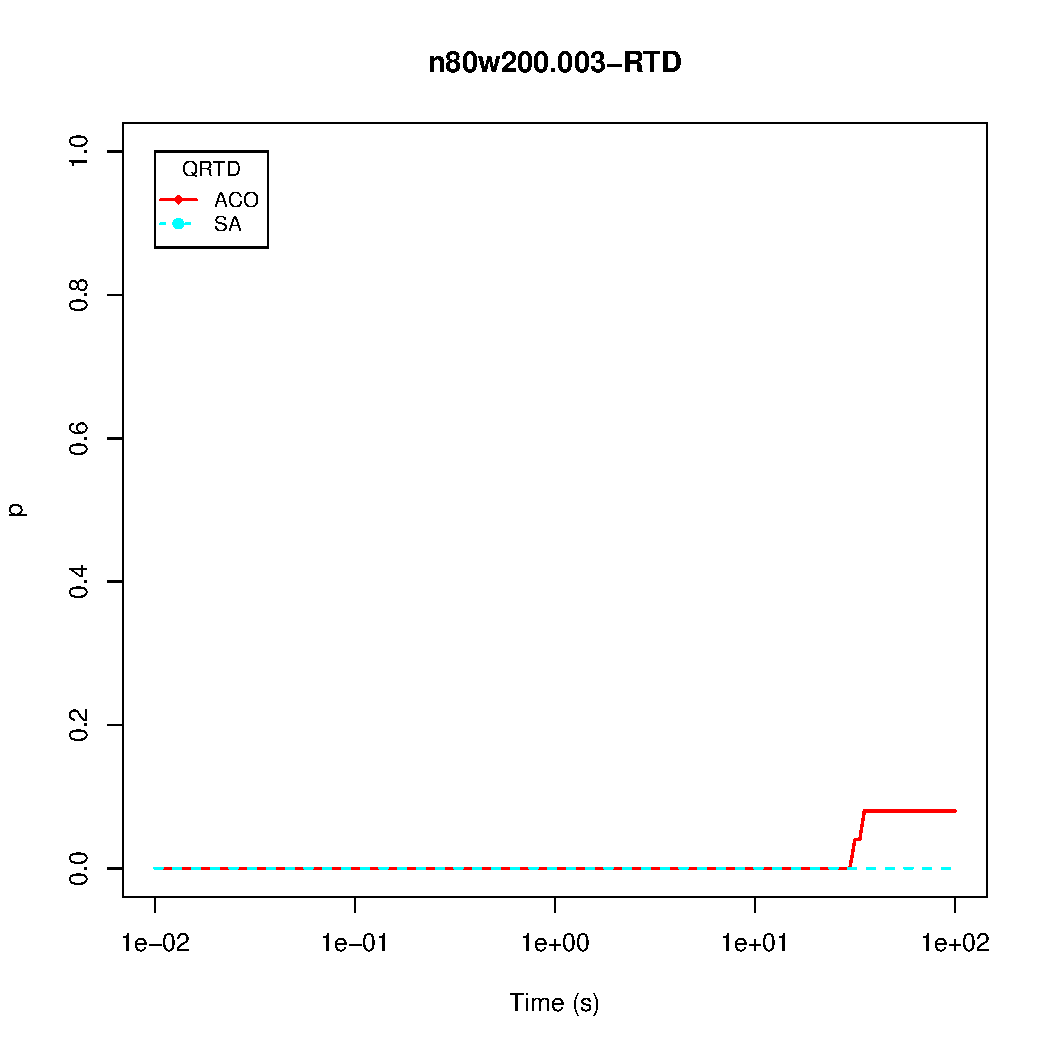
\includegraphics[width=0.6\textwidth,keepaspectratio]{{SLS/n80w200.003/n80w200.003-RTDs}.pdf}
\captionof{figure}{n80w200.003 - Run-time distribution plots of the implemented algorithms for $q* = 0.02$}
\end{center}

\begin{center}
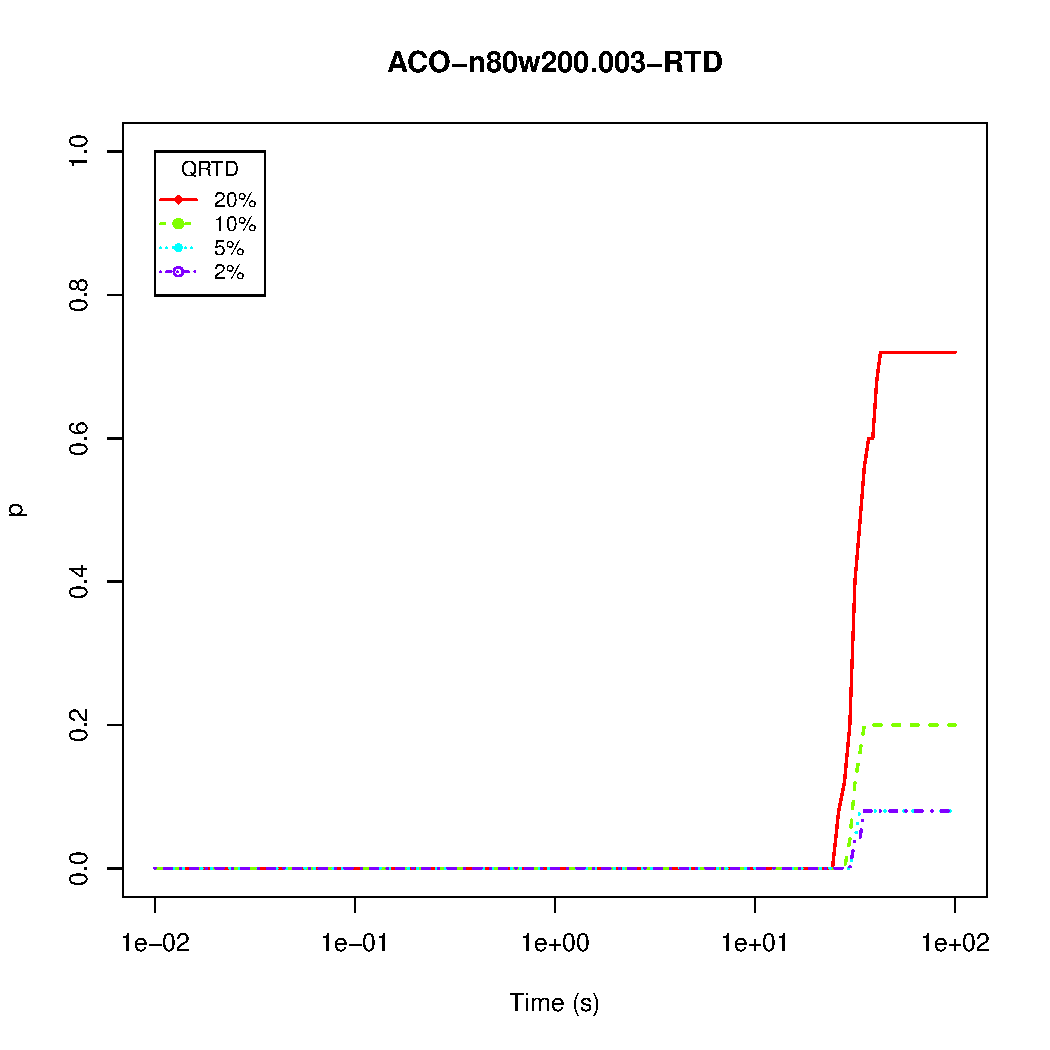
\includegraphics[width=0.6\textwidth,keepaspectratio]{{SLS/n80w200.003/ACO-n80w200.003-RTDs}.pdf}
\captionof{figure}{n80w200.003 - Run-time distribution plots of the ACO algorithm for different values of $q*$}
\end{center}

\begin{center}
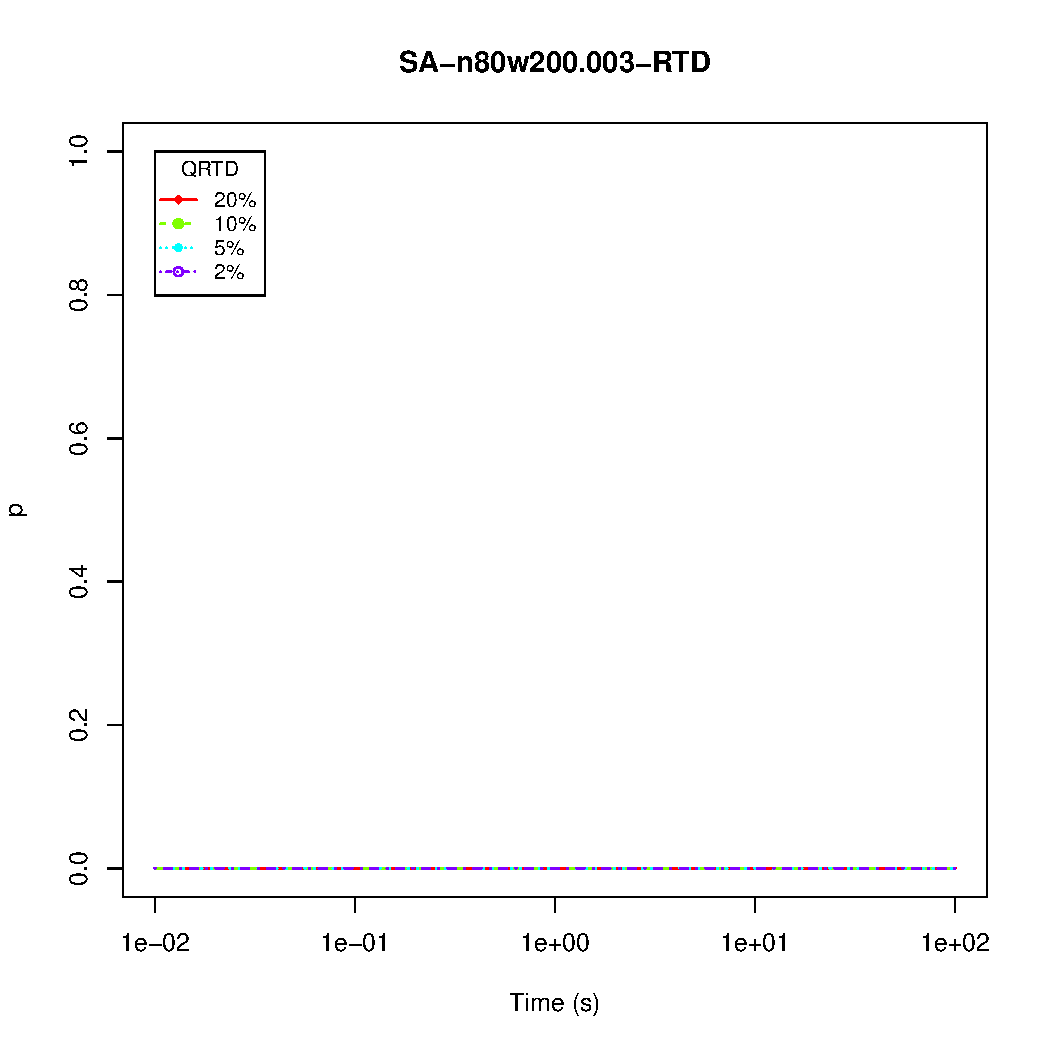
\includegraphics[width=0.6\textwidth,keepaspectratio]{{SLS/n80w200.003/SA-n80w200.003-RTDs}.pdf}
\captionof{figure}{n80w200.003 - Run-time distribution plots of the SA algorithm for different values of $q*$}
\end{center}

\subsubsection{n80w200.004}
\begin{center}
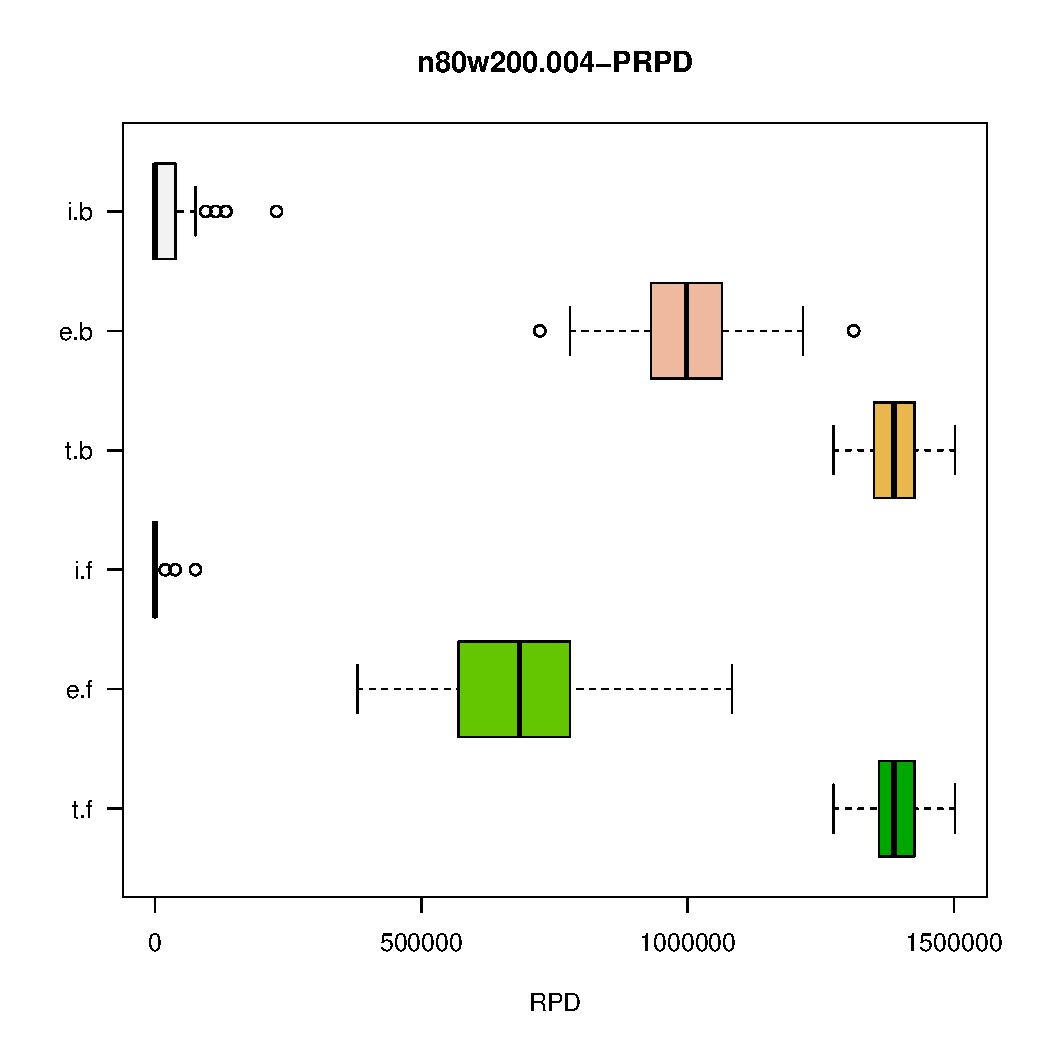
\includegraphics[width=0.6\textwidth,keepaspectratio]{{SLS/n80w200.004/n80w200.004-PRPD}.pdf}
\captionof{figure}{n80w200.004 - Penalised Relative Percentage Deviation box-plot for the implemented SLS algorithms}
\end{center}

\begin{center}
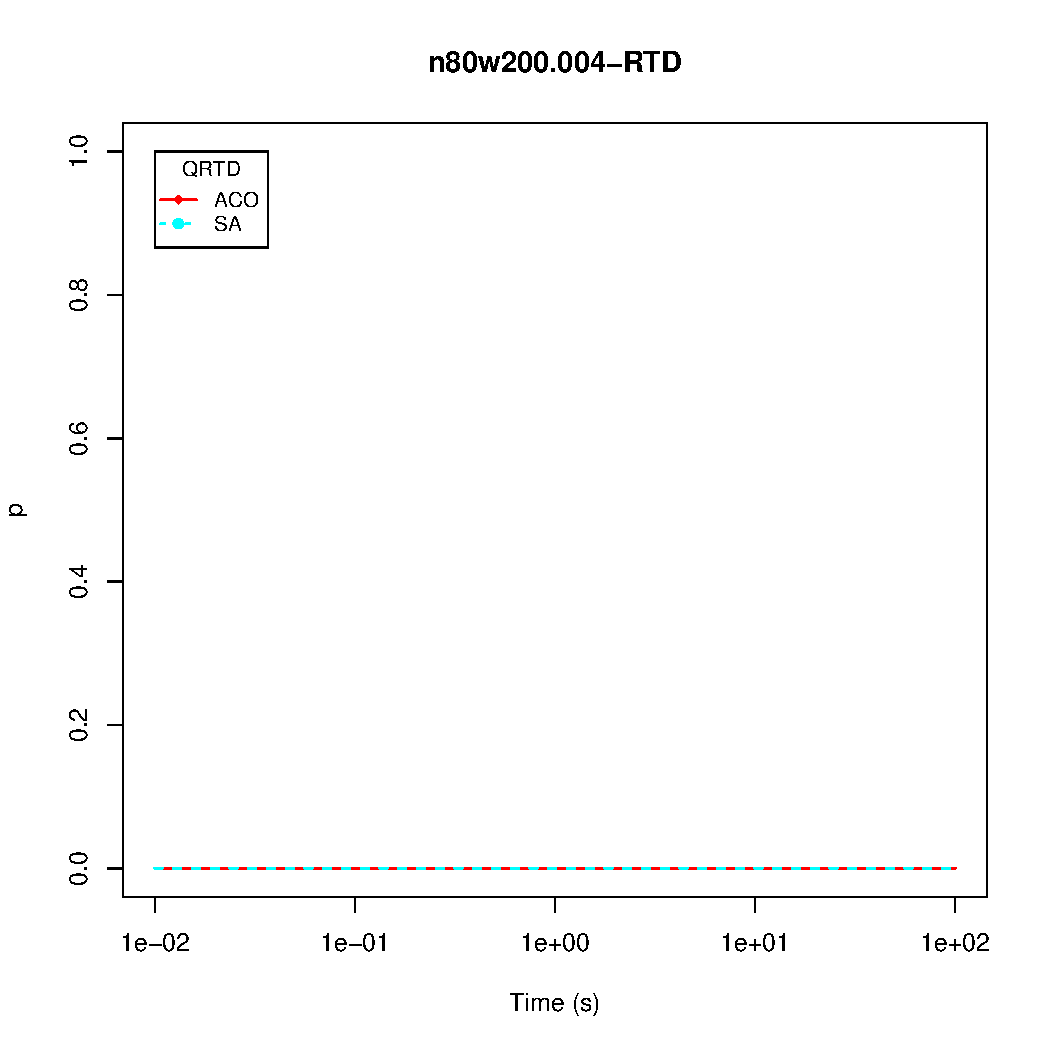
\includegraphics[width=0.6\textwidth,keepaspectratio]{{SLS/n80w200.004/n80w200.004-RTDs}.pdf}
\captionof{figure}{n80w200.004 - Run-time distribution plots of the implemented algorithms for $q* = 0.02$}
\end{center}

\begin{center}
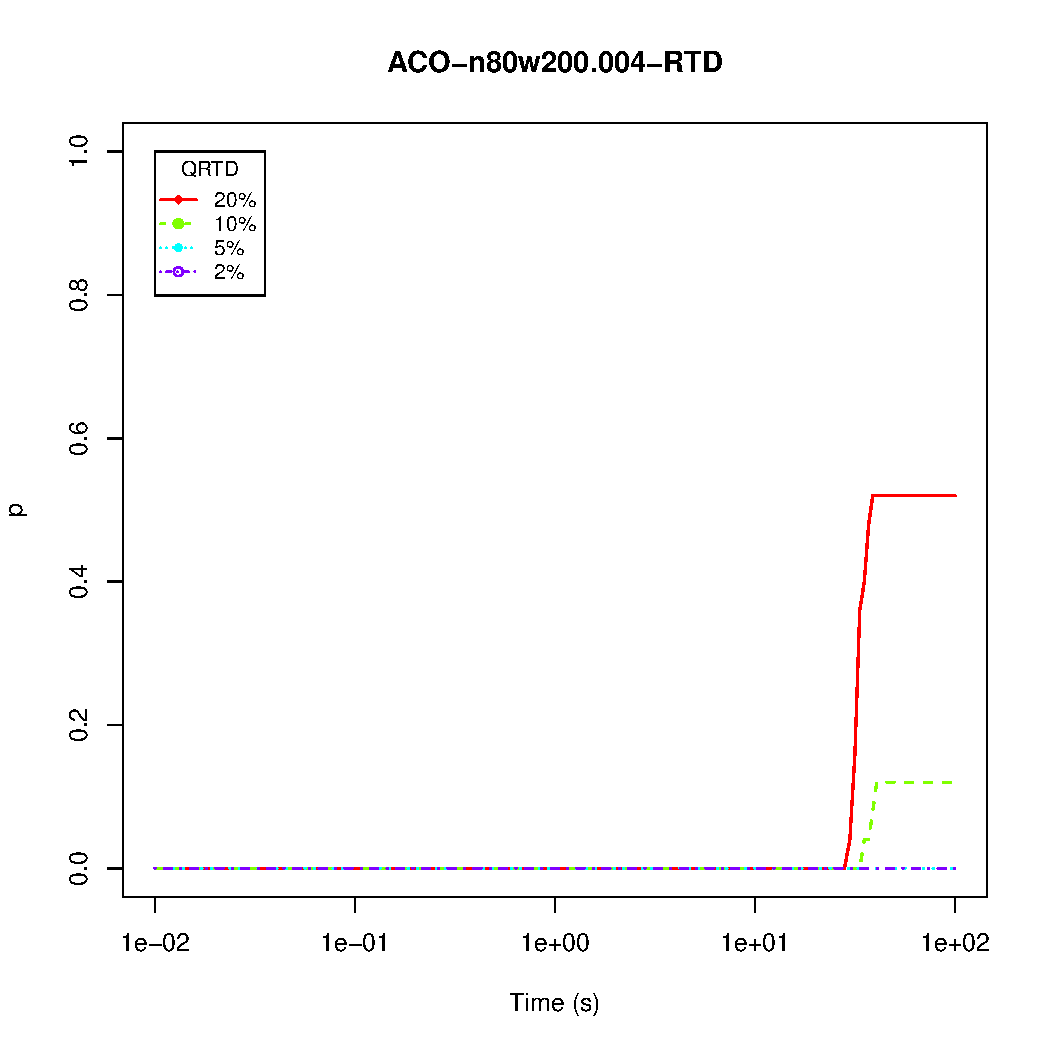
\includegraphics[width=0.6\textwidth,keepaspectratio]{{SLS/n80w200.004/ACO-n80w200.004-RTDs}.pdf}
\captionof{figure}{n80w200.004 - Run-time distribution plots of the ACO algorithm for different values of $q*$}
\end{center}

\begin{center}
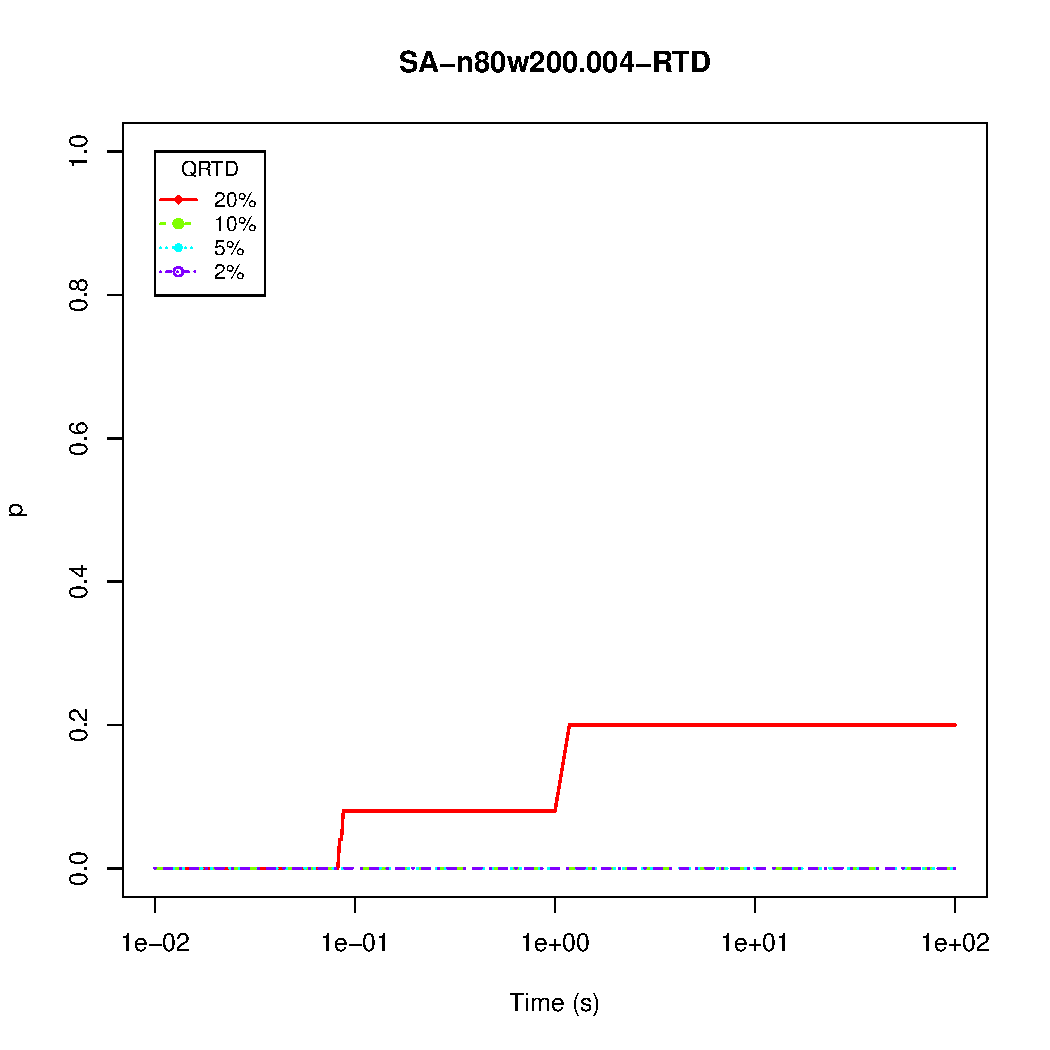
\includegraphics[width=0.6\textwidth,keepaspectratio]{{SLS/n80w200.004/SA-n80w200.004-RTDs}.pdf}
\captionof{figure}{n80w200.004 - Run-time distribution plots of the SA algorithm for different values of $q*$}
\end{center}

\subsubsection{n80w200.005}
\begin{center}
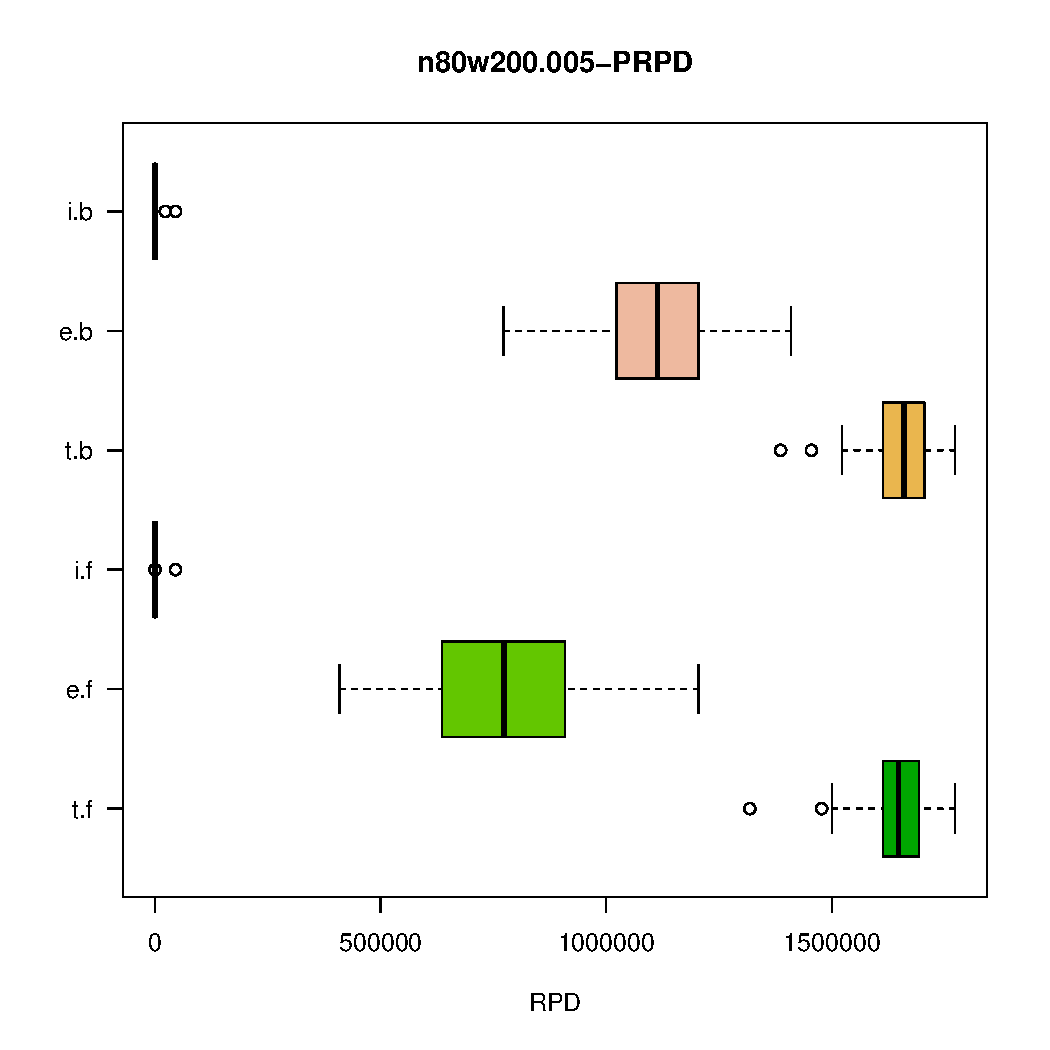
\includegraphics[width=0.6\textwidth,keepaspectratio]{{SLS/n80w200.005/n80w200.005-PRPD}.pdf}
\captionof{figure}{n80w200.005 - Penalised Relative Percentage Deviation box-plot for the implemented SLS algorithms}
\end{center}

\begin{center}
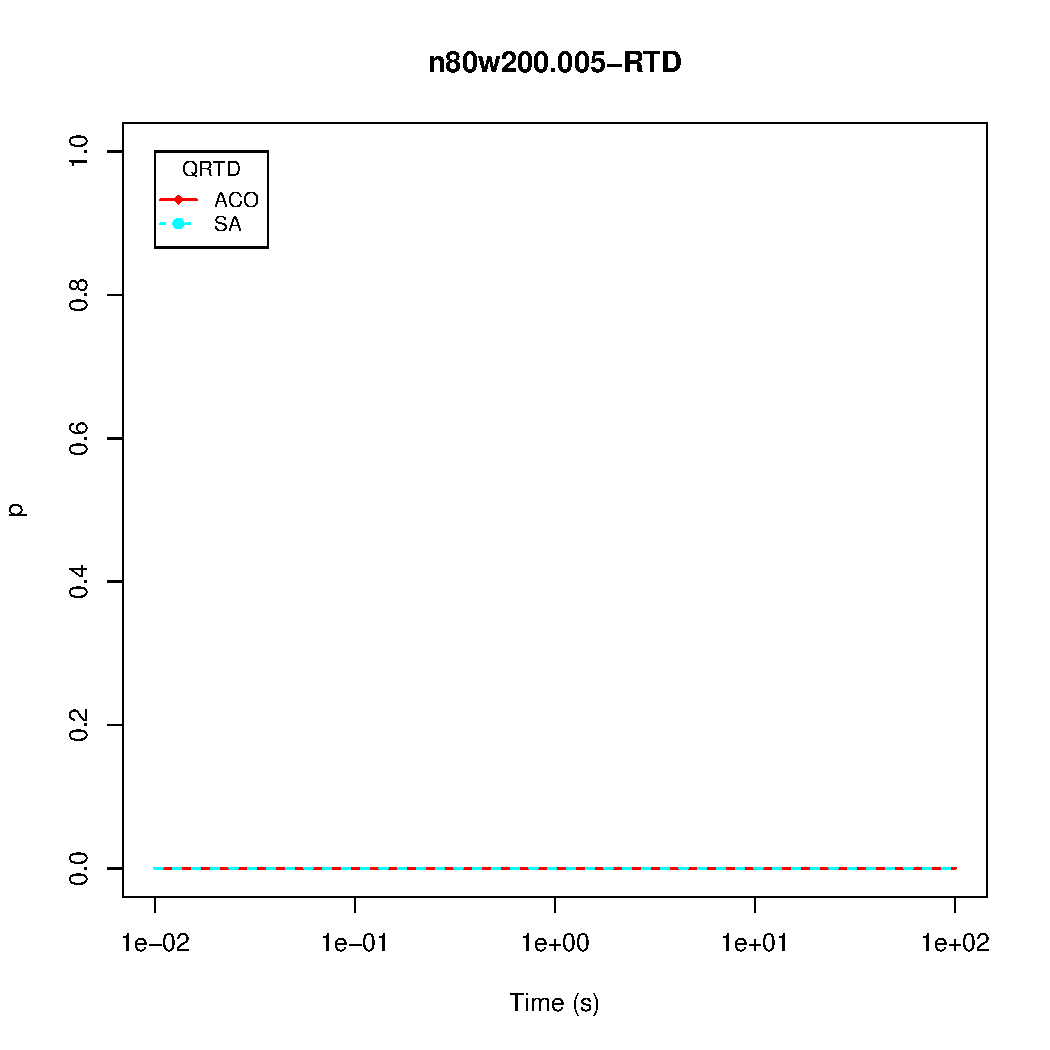
\includegraphics[width=0.6\textwidth,keepaspectratio]{{SLS/n80w200.005/n80w200.005-RTDs}.pdf}
\captionof{figure}{n80w200.005 - Run-time distribution plots of the implemented algorithms for $q* = 0.02$}
\end{center}

\begin{center}
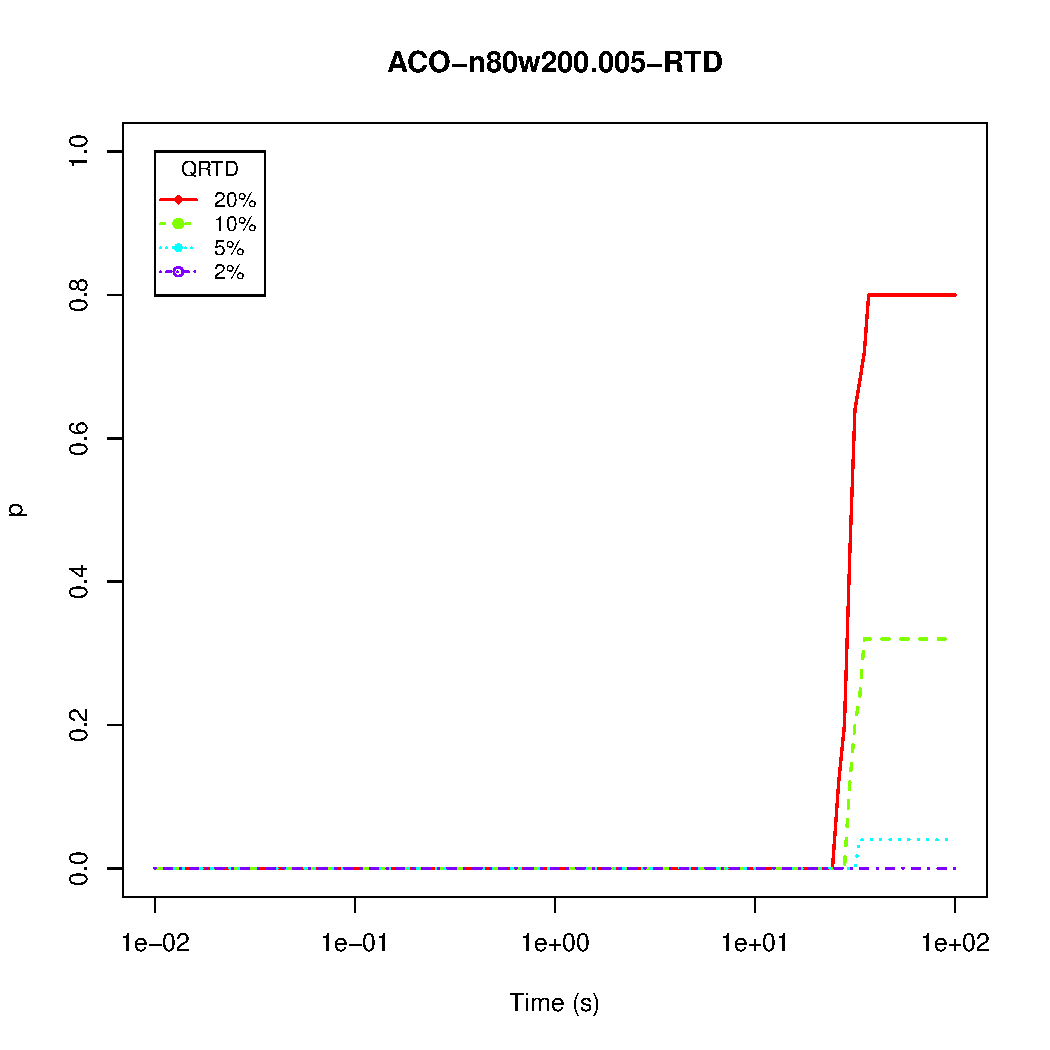
\includegraphics[width=0.6\textwidth,keepaspectratio]{{SLS/n80w200.005/ACO-n80w200.005-RTDs}.pdf}
\captionof{figure}{n80w200.005 - Run-time distribution plots of the ACO algorithm for different values of $q*$}
\end{center}

\begin{center}
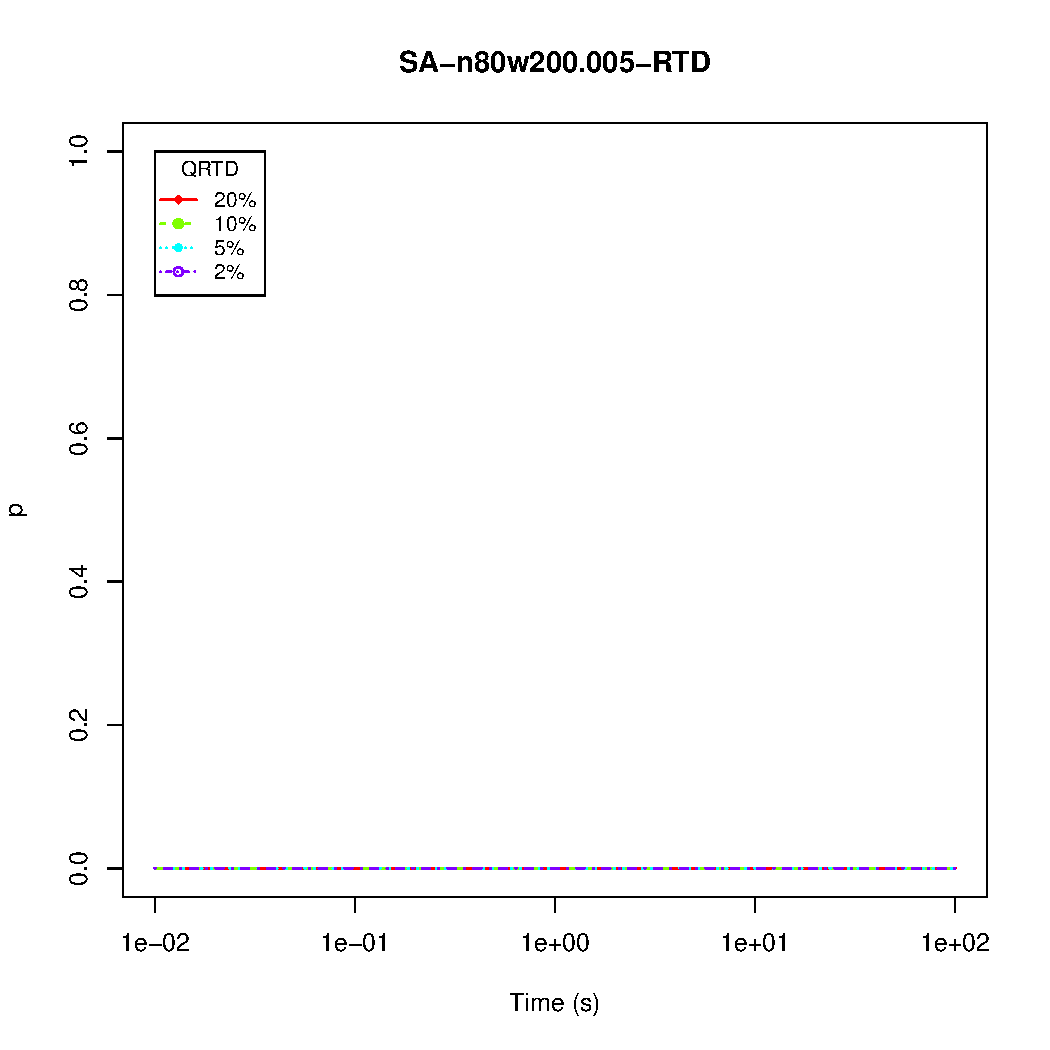
\includegraphics[width=0.6\textwidth,keepaspectratio]{{SLS/n80w200.005/SA-n80w200.005-RTDs}.pdf}
\captionof{figure}{n80w200.005 - Run-time distribution plots of the SA algorithm for different values of $q*$}
\end{center}

\subsection{Results discussion}
Before starting the results analysis one should note that the maximum run-time of the algorithm should be chosen to allow for long enough run of the SLS.
  
The proposed maximum run-time is equal to $10 \cdot 1000 \cdot runtime(VND)$, which in the worst case, for the proposed algorithms, will be equal to $60000s$.
  
In order to have reasonable computation times for the whole set of instances, the maximum run-time has been set to $100s$.
  
This choice has a strong influence on the quality of the solution generated by the algorithm.

\paragraph{Solution quality}

By looking at tables \ref{tab:acostat} and \ref{tab:sastat} one can see that:
\begin{itemize}

\item The conclusions that can be drawn by observing the percentage of infeasible runs and the average penalized relative percentage deviation may seem conflicting at first sight. 
This is due to the fact that unfeasible solutions have a great impact on the average PRPD because of the magnitude of the penalization related to constraint violations.

\item Both algorithms are more effective on the $n80w200.X$ instances than the $n80w20.X$ ones, since they have a lower percentage of infeasible runs and a lower PRPD.

\item As in the previous implementation exercise, instance $n80w20.002$ appears to be the most difficult one for both the algorithm, since the PRPD distribution is centered around 12000-15000, thus indicating the presence of constraint violations in the best found solution.

This result is confirmed by a percentage of unfeasible solution greater than 80\% for both the algorithms.

\item Instances $n80w20.003$ and $n80w20.004$ are also particularly difficult to solve for both the algorithms, as the higher percentage of unfeasible solutions shows.

Moreover, by looking at the box-plots, one can see that both the distributions are centered on values higher than 20000, thus indicating an high number of constraint violations in most of the simulations.


\item The SA algorithm is able to generate more feasible solution than the ACO one on almost all the instances, the only exception being instance $n80w20.002$.

\item Furthermore, by looking at the PRPD, namely its average value and its distribution, represented by means of a box-plot, one can see that the penalized relative percentage deviation of the solutions generated by the SA algorithm is generally lower than the solutions generated by the ACO one.
ACO algorithm reaches higher quality solutions only on instances $n80w20.002$ and $n80w200.005$.

% \item For some other instances (e.g. $n80w20.004$,$n80w20.005$) the algorithms are able to converge to feasible solutions and to the best-known one, but having a right-skewed distribution towards higher values of PRPD.

% \item For the remaining instances, except for some outlier values, the algorithms are able to converge to the best-known solution in most of the runs , even though the average PRPD is not closer to 0. This is due to the fact that the mean of a distribution is sensible to outliers and the penalisation for a constraint violations is extremely high when compared to the mean value.
      
% \item The algorithm ordering in terms of runtimes is $s.tie < p.tie < p.tei < s.tei$ for the  $n80w20.X$ instances while $s.tie < p.tei < s.tei < p.tie$ for $n80w200.X$ ones. The choice to explore the Insert Neighborhood before the Exchange one allows to reduce the computation time for the $n80w20.X$ instances, with a similar solution quality.

% \item The algorithms are more effective on the $n80w200.X$ instances then the $n80w20.X$ once, since they have a lower percentage of infeasible runs and a lower PRPD.

% \item The standard variable neighborhood descent with Transpose-Insert-Exchange neighborhood chain (s.tie) outperforms all the other algorithms in terms of solution quality and runtime.

\item Table \ref{tab:wilcoxon} contains, for each analyzed problem instance, p-values considerably smaller than the significance level ($\alpha=0.05$). 

This implies that the null hypothesis corresponding to the equality of the median values of the differences of the two distributions can be rejected, hence assessing the existence of a statistically significant difference among the solution quality generated by the implemented algorithms.

% \item By looking at the Cpu time, one can see that the instances \emph{n80w20.X} have generally lower runtimes than the \emph{n80w200.X} ones. They can then be considered, with respect to the variable neighborhood descent algorithms, simpler (quickier to solve) instances with respect to the latter.

\end{itemize}

\subsection{Run-time distribution}
By looking at the qualified run-time distribution plots one can see that:
\begin{itemize}

\item No run-time distribution is able to reach a success probability of 1.

On the majority of the instances, this can also be deduced by looking at the percentage of unfeasible runs in \ref{tab:acostat}, \ref{tab:sastat}. 

Due to the penalization on constraint violations, a solution must be feasible in order to have an high quality, hence a non null percentage of unfeasible solution will necessarily imply that it would be impossible to reach an high solution quality on all the runs.  

\item Both the algorithms are able to reach an higher percentage of feasible solutions on the $n80w200.X$ instances than on the $n80w20.X$ ones, but no algorithm is able to generate high quality solutions ($q_r < 0.02$) on any of the $n80w200.X$ instances.

\item On the other hand, on the $n80w20.X$ set, the SA algorithm is able to generate high quality solutions with an high probability with a smaller run-time than the ACO algorithm.

Again, the only exception is the $n80w20.002$ instance.

\item However, if one considers higher values of $q^{*}$, one can see that the ACO algorithm is able to find solutions having a better quality than those generated by the SA one on the $n80w200.X$ set.

\item The run-time distribution plots comparing the distributions for different quality thresholds ($q^{*}$) shows that even by relaxing the bound up to 20\% a success probability of 1 cannot be attained.

This shows that both of the algorithms tends to converge to feasible but sub-optimal solutions.

\item The probability of finding high quality solutions, on all the instances, has a steep increase around $1s$ for the SA algorithm and around $30s$ for the ACO one.
 
\end{itemize}
